% You can choose whether you prefer a single or double column appendix.
% Whatever you choose, you will need to stick to it throughout the appendix.
% For double column style, comment the next line.
\onecolumn

\appendix
\begin{appendices}

\section{Acknowledgements}
\label{appendix:acknowledgements}

My sincere gratitude to all the participants who generously contributed to this research by dedicating their valuable time to respond to the questionnaires voluntarily, as well as the participants who willingly tested and interacted with prototypes created for this research for their feedback and evaluation through interviews. Additionally, I thank everyone who supported me in the data gathering and prototyping phase by providing hardware, testing, and debugging code.

Special appreciation goes to Shruti Rao Ph.D. Candidate (University of Amsterdam) for her constructive feedback and suggestions, which further expanded this research, and internal supervisor Dr. Hamed S. Alavi (University of Amsterdam), for his invaluable guidance and thought-provoking questions throughout the project. Also, my sincere appreciation to all the reviewers of this research, particularly drafts of this paper, for their insightful comments and contributions.

\section{Ethical considerations}
\label{appendix:ethical}

Before user studies and data gathering were conducted, an application to the Ethics Committee for Information Sciences (ECIS) \footnote{https://ivi.uva.nl/research/ethical-code/ethical-code.html} was made. No ethical issues were raised and the committee gave positive advice before the start of the research. All individuals participating in the questionnaire and evaluation process were obliged to confirm their voluntary involvement by carefully reading and submitting consent forms, with the assurance that they retained the right to withdraw from participation at any point without the need for explanation.

Participants were informed about the goal of the study and the structure of the interviews. Participants were not (financially) incentivized to take part in the studies. To uphold confidentiality and privacy, questionnaire participation occurred anonymously, and all evaluation interview data underwent anonymization following the conclusion of the evaluation sessions. Interacting with occupants within the building and interacting with participants of the usability tests of the prototype adhered to the principles outlined in the University of Amsterdam Code of Conduct \footnote{https://www.uva.nl/en/about-the-uva/policy-and-regulations/} and Campus rules and Policies \footnote{https://extranet.uva.nl/en/content/a-z/house-rules-and-code-of-conduct/house-rules-and-code-of-conduct.html}.

\section{Domain Expert Validity and Pilot Tests}
\label{appendix:experts}

Before conducting the questionnaire survey, data gathering process, and interview evaluation procedures, domain experts from the Informatics Institute \footnote{https://ivi.uva.nl/} and the Digital Interactions Lab (DIL) \footnote{https://uva-dilab.com/} at the University of Amsterdam reviewed the methodology procedures. Draft versions of the questions and techniques were sent out to the supervisors and researchers from the lab for feedback internally. Then the questionnaire survey and evaluation interview procedure were pilot-tested and after several iterations more widely distributed to occupants and open for participation. The research was presented during two internal 'lab meetings'. First, a brainstorming workshop was held with the concept diagrams of the prototype for expert review and second, the final proof-of-concept prototype was presented for feedback and design improvements. 

\section{Data storage and archival}
\label{appendix:data}

During the research phase data collection methods, storage, and archival followed the Central guidelines for research data management (RDM) \footnote{https://rdm.uva.nl/en/introduction/rdm-introduction.html} from the University of Amsterdam. All occupant data was anonymized before publishing and nothing that can be considered personal data is collected. Data is stored on cloud service providers provided by the University of Amsterdam such as Research Drive \footnote{https://rdm.uva.nl/en/looking-after/storage/storage.html}. Only the principal researcher and supervisor(s) in possession of the encryption methods and passwords can view the unstructured exported data from the questionnaires, monitoring devices, and interviews. Only aggregated datasets and data outputs for the purpose of visualization are published and can be publicly viewed.

\section{Prototype budget and costs}
\label{appendix:ethical}

Some of the hardware components and materials were bought specifically for the creation of the prototype. These costs were declared to the Digital Interactions Lab (DIL) and deducted from the lab budget. All other components were already in possession of the researcher. The author(s) has no affiliation with any of the hardware companies and organizations mentioned in this paper and received no other financial support for the creation of the prototype.

\section{Source code and datasets}
\label{appendix:source}

In the spirit of Open Access Research \footnote{https://uba.uva.nl/en/support/research/open-access/open-access.html}, to support reproducibility, mitigate a lack of transparency, and enable future work in this research field the aggregated datasets, notebooks, and prototype source code in this research are publicly available on a GitHub organization with the working title 'viszlab' using the MIT License. Several code repositories for different parts of the research can be accessed and publicly viewed. The README file of each repository describes the contents and how to perform the technical set-up: \underline{https://github.com/viszlab/}

\pagebreak

\section{Floorplan and lab set-up}
\label{appendix:floorplan}

A floorplan diagram (see \hyperref[fig:floorplan]{Figure \ref{fig:floorplan}}) providing an overview of the technical lab setup of the small (Room A) and large (Room B) meeting rooms used for indoor air quality monitoring. The floorplan indicates the position the monitors are installed and the position of doors and windows.

\begin{figure}[H]
    \centering
    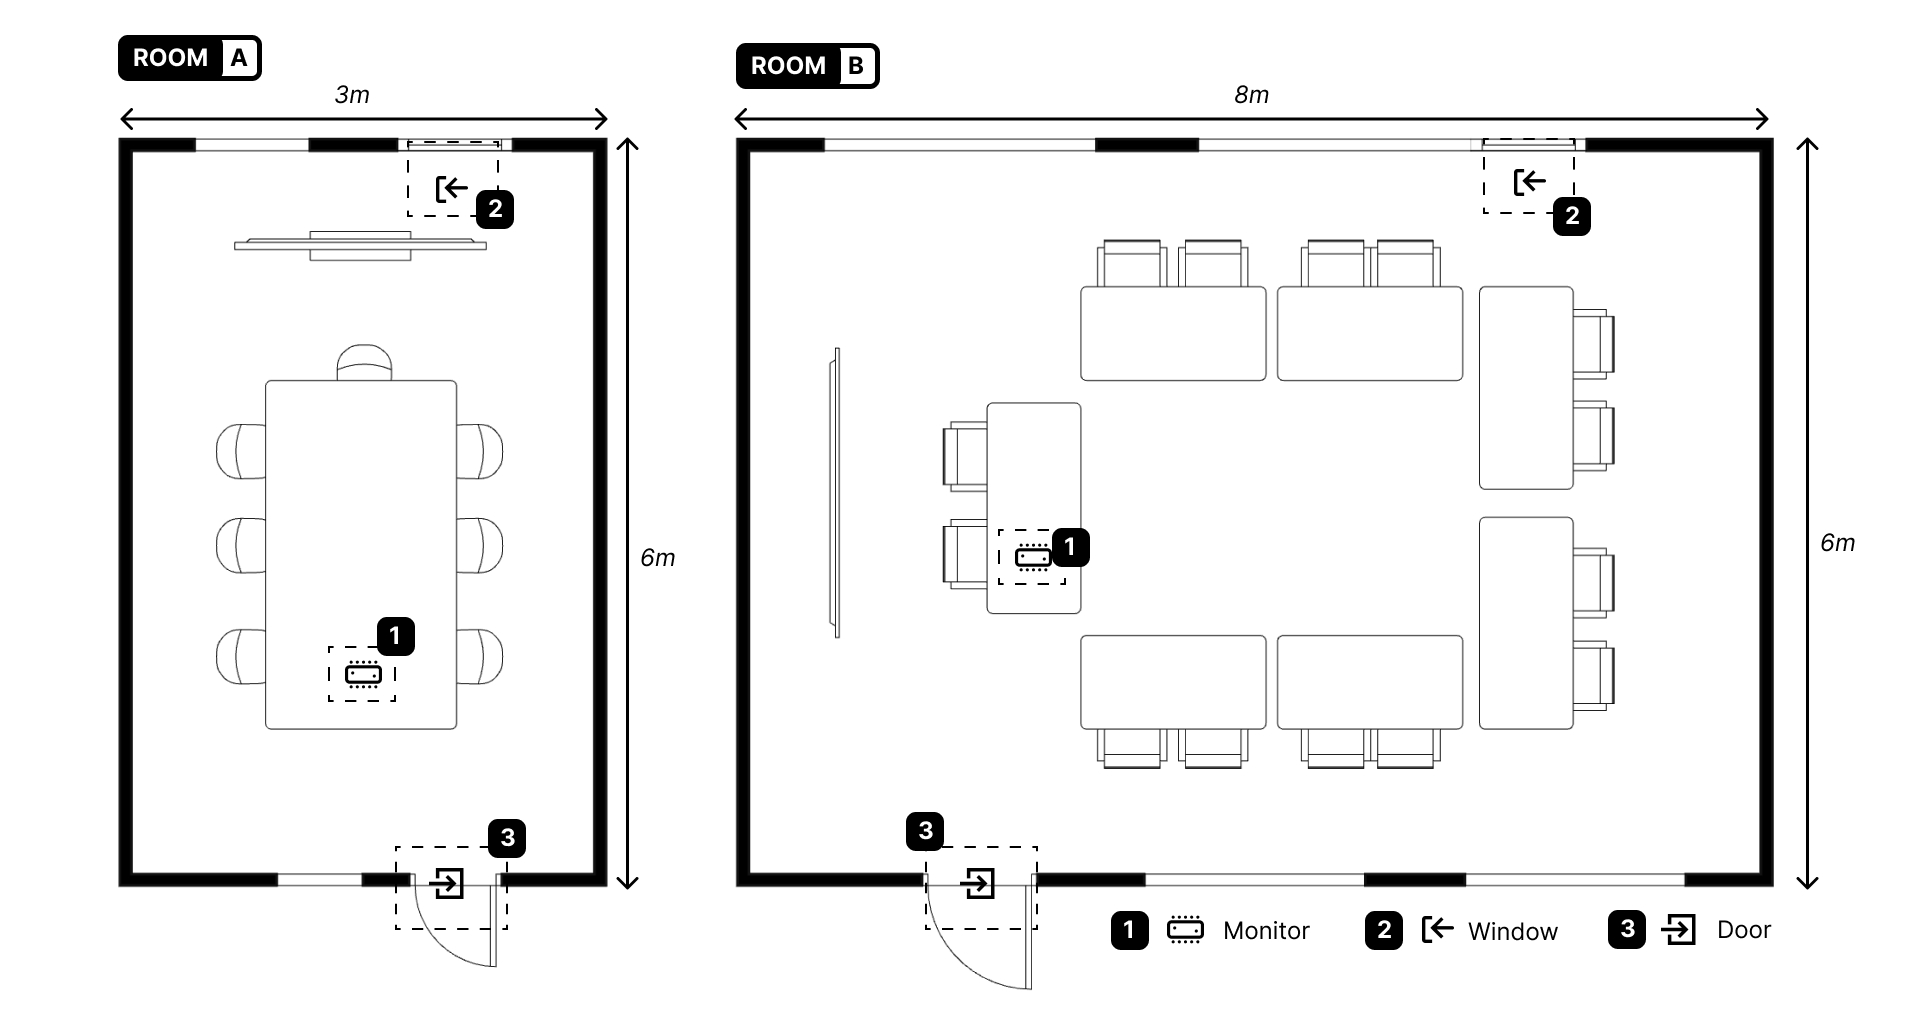
\includegraphics[width=0.8\paperwidth]{meeting_rooms_floorplan.jpg}
    \caption{Floorplan of Room A and B, monitors installed as of manufacturer specifications}
    \label{fig:floorplan}
\end{figure}

\section{Meeting room impressions}
\label{appendix:meetings}

Photographs of the small (Room A, see \hyperref[fig:room-a]{Figure \ref{fig:room-a}}) and large (Room B, see \hyperref[fig:room-b]{Figure \ref{fig:room-b}}) meeting rooms taken from the viewpoint of the entrance of the door. It shows the default interior design set-up of the rooms and the position of the chairs and tables.

\begin{figure}[H]
\begin{minipage}{.5\textwidth}
    \centering
    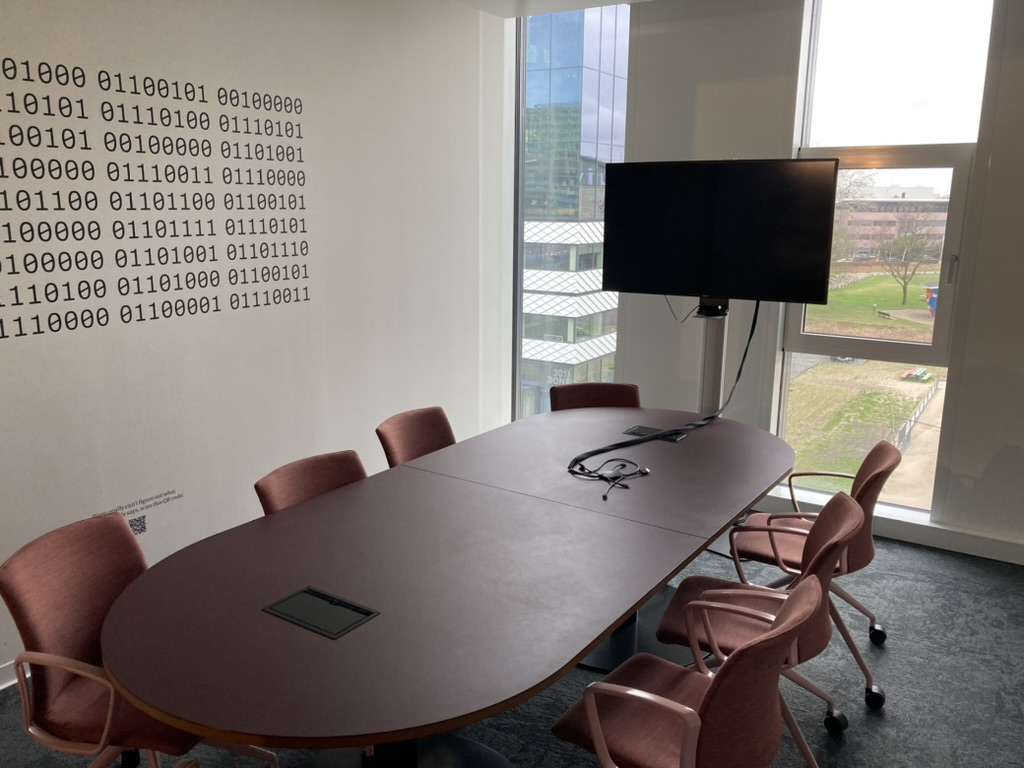
\includegraphics[width=85mm,height=70mm]{photograph-room-a.jpeg}
    \caption{The 'smaller'(18$m2$) space labeled Room A}
    \label{fig:room-a}
\end{minipage}%
\begin{minipage}{.5\textwidth}
    \centering
    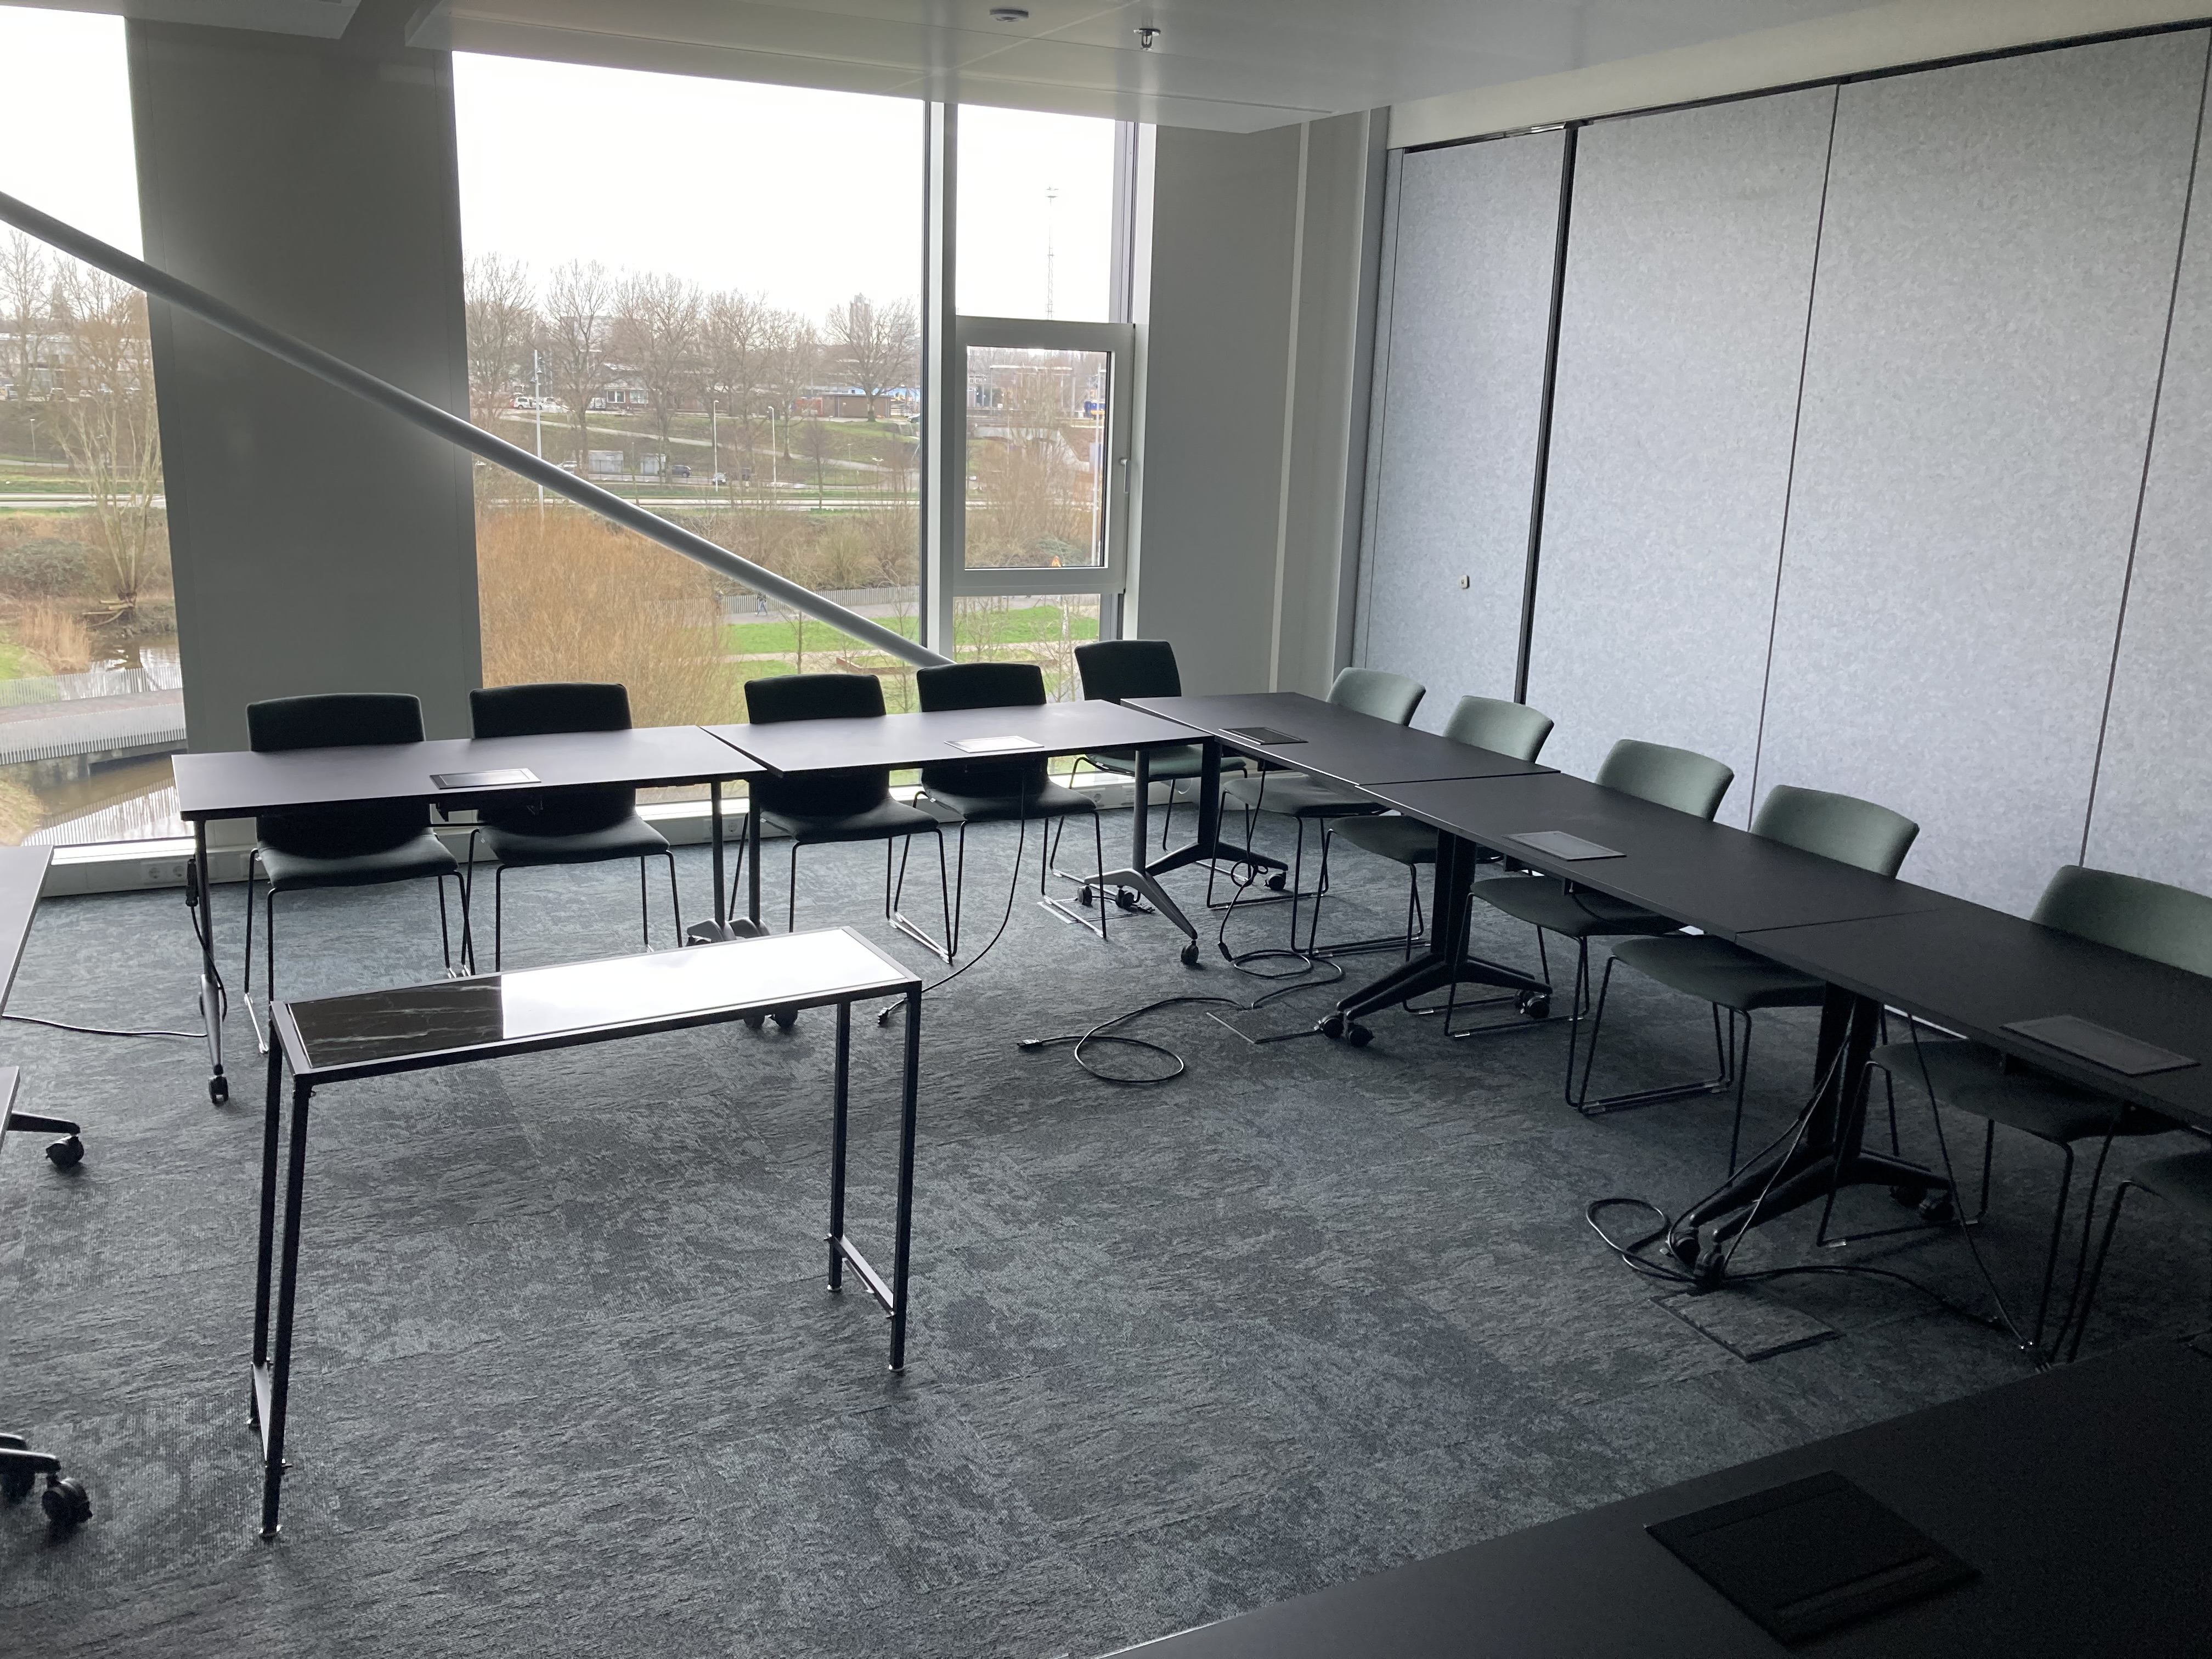
\includegraphics[width=85mm,height=70mm]{photograph-room-b.jpeg}
    \caption{The 'larger' (48$m2$) space labeled Room B}
    \label{fig:room-b}
\end{minipage}%
\end{figure}

\section{Building impressions}
\label{appendix:building}

Photographs of the Lab42 building interior and exterior. The buildings's layout is strategically organized into different zones, each serving various functions, ranging from quiet individual work to spaces that allow for collaborative work. Lecture halls, learning rooms, and open learning spaces make up the two lower floors, with the upper four being primarily assigned to the university academic staff, meeting rooms, and external offices. The overarching interior theme in the design revolves around 'tech' and 'nature' aiming to cultivate a fresh, light, and warm comfortable ambiance. 

\begin{figure}[htbp]
    \centering
    \begin{subfigure}{0.48\textwidth}
        \centering
        
\includegraphics[width=\textwidth]{placeholder-two.jpg}
        \caption{Placeholder}
        \label{fig:image1}
    \end{subfigure}
    \hfill
    \begin{subfigure}{0.48\textwidth}
        \centering
        
\includegraphics[width=\textwidth]{placeholder-two.jpg}
        \caption{Placeholder}
        \label{fig:image2}
    \end{subfigure}
    \caption{Placeholder}
    \label{fig:grid}
\end{figure}

\begin{figure}[htbp]
    \centering
    \begin{subfigure}{0.48\textwidth}
        \centering
        
\includegraphics[width=\textwidth]{placeholder-two.jpg}
        \caption{Placeholder}
        \label{fig:image1}
    \end{subfigure}
    \hfill
    \begin{subfigure}{0.48\textwidth}
        \centering
        
\includegraphics[width=\textwidth]{placeholder-two.jpg}
        \caption{Placeholder}
        \label{fig:image2}
    \end{subfigure}
    \caption{Placeholder}
    \label{fig:grid}
\end{figure}

\begin{figure}[htbp]
    \centering
    \begin{subfigure}{0.48\textwidth}
        \centering
        
\includegraphics[width=\textwidth]{placeholder-two.jpg}
        \caption{Placeholder}
        \label{fig:image1}
    \end{subfigure}
    \hfill
    \begin{subfigure}{0.48\textwidth}
        \centering
        
\includegraphics[width=\textwidth]{placeholder-two.jpg}
        \caption{Placeholder}
        \label{fig:image2}
    \end{subfigure}
    \caption{Placeholder}
    \label{fig:grid}
\end{figure}

\section{Prototype impressions}
\label{appendix:prototype}

Photographs of the prototype-creating phase showing the manufacturing of the pulley mechanism (see \hyperref[fig:prototype-pulley]{Figure \ref{fig:prototype-pulley}}), fabricating the leaves (see \hyperref[fig:prototype-leaves]{Figure \ref{fig:prototype-leaves}}) and mounting the electronics (see \hyperref[fig:prototype-board]{Figure \ref{fig:prototype-board}}) for the high fidelity data physicalization prototype.

\begin{figure}[htbp]
    \centering
    \begin{subfigure}{0.48\textwidth}
        \centering
        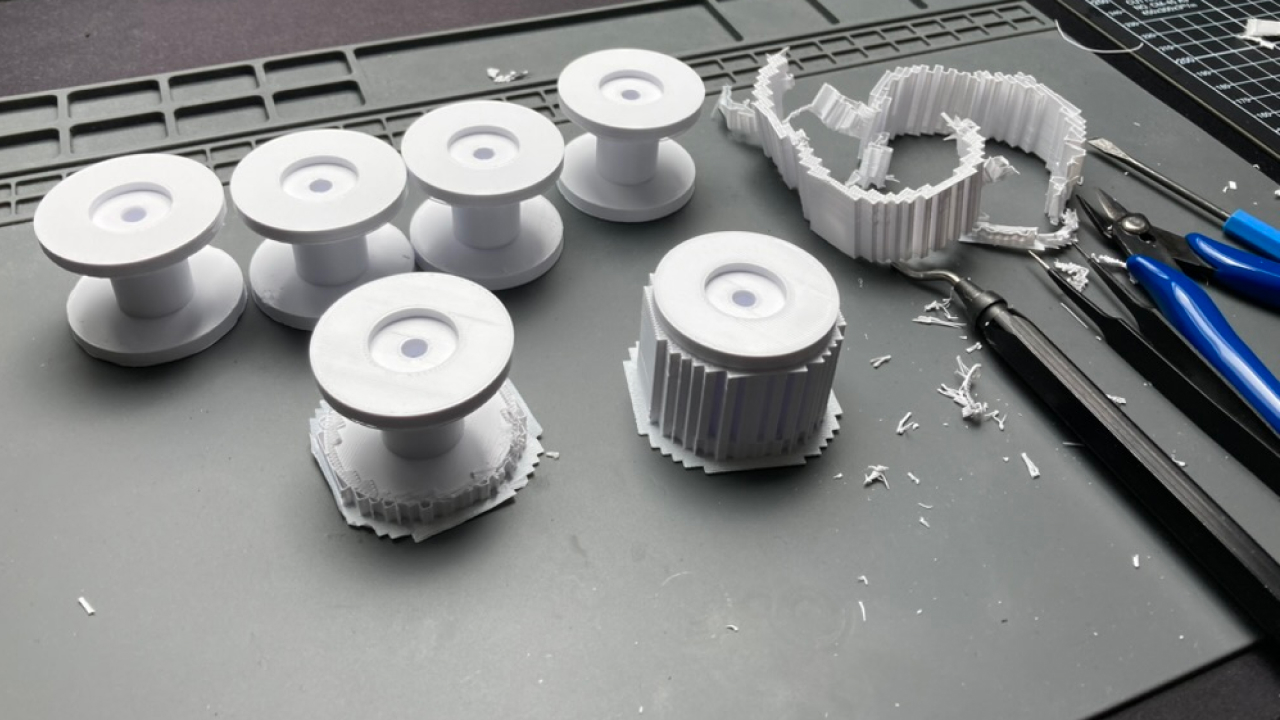
\includegraphics[width=\textwidth]{prototype_pulley_printing.jpg}
        \caption{Cleaning and sanding the 3D printed pulleys}
        \label{fig:pulley-sanding}
    \end{subfigure}
    \hfill
    \begin{subfigure}{0.48\textwidth}
        \centering
        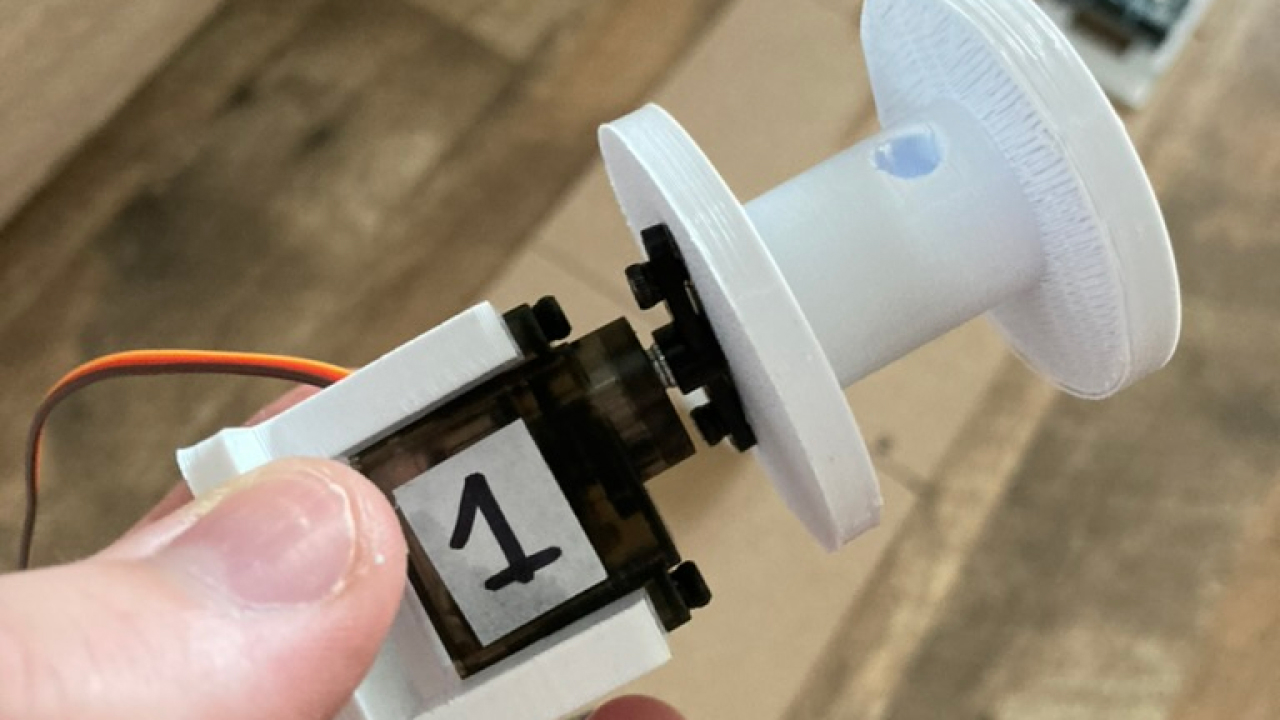
\includegraphics[width=\textwidth]{prototype_pulley_servo.jpg}
        \caption{Attaching pulleys to servo motors using motor arms}
        \label{fig:pulley-servo}
    \end{subfigure}
    \caption{The pull-up and down mechanism of the hanging planter strings}
    \label{fig:prototype-pulley}
\end{figure}

\begin{figure}[htbp]
    \centering
    \begin{subfigure}{0.48\textwidth}
        \centering
        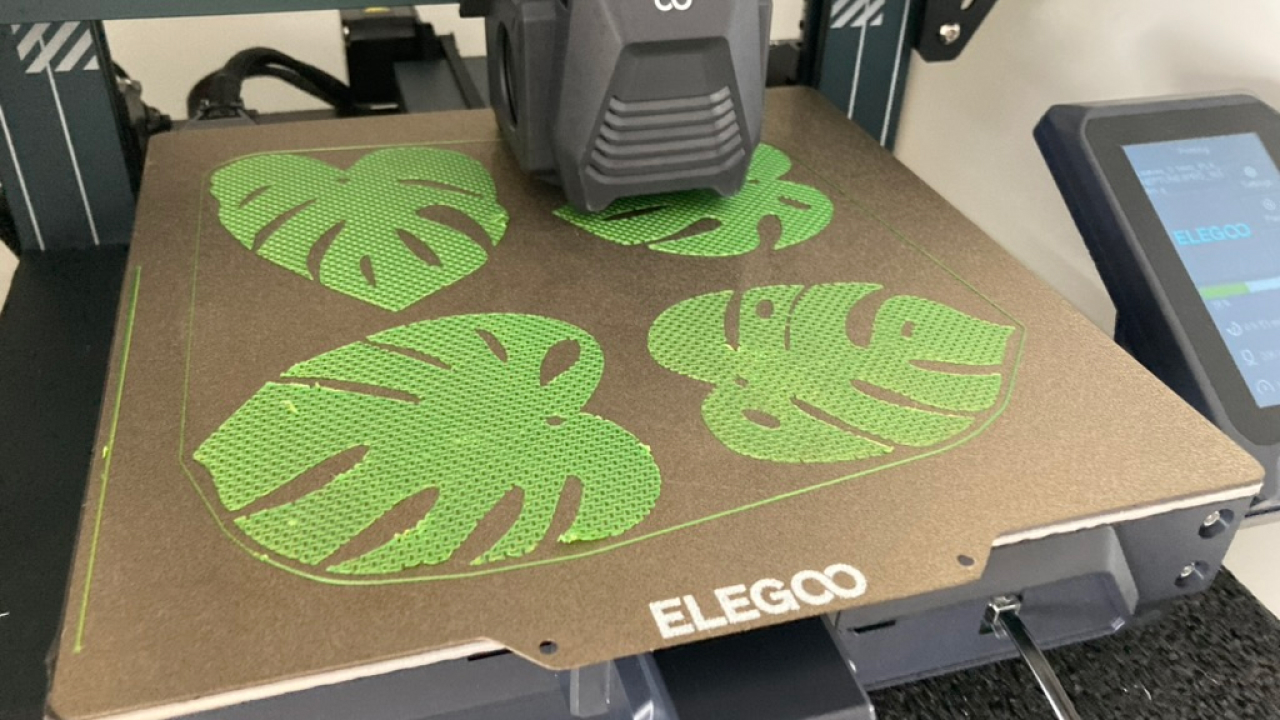
\includegraphics[width=\textwidth]{prototype_printing_leaves.jpg}
        \caption{FDM 3D printer printing the textile leaves}
        \label{fig:printing-leaves}
    \end{subfigure}
    \hfill
    \begin{subfigure}{0.48\textwidth}
        \centering
        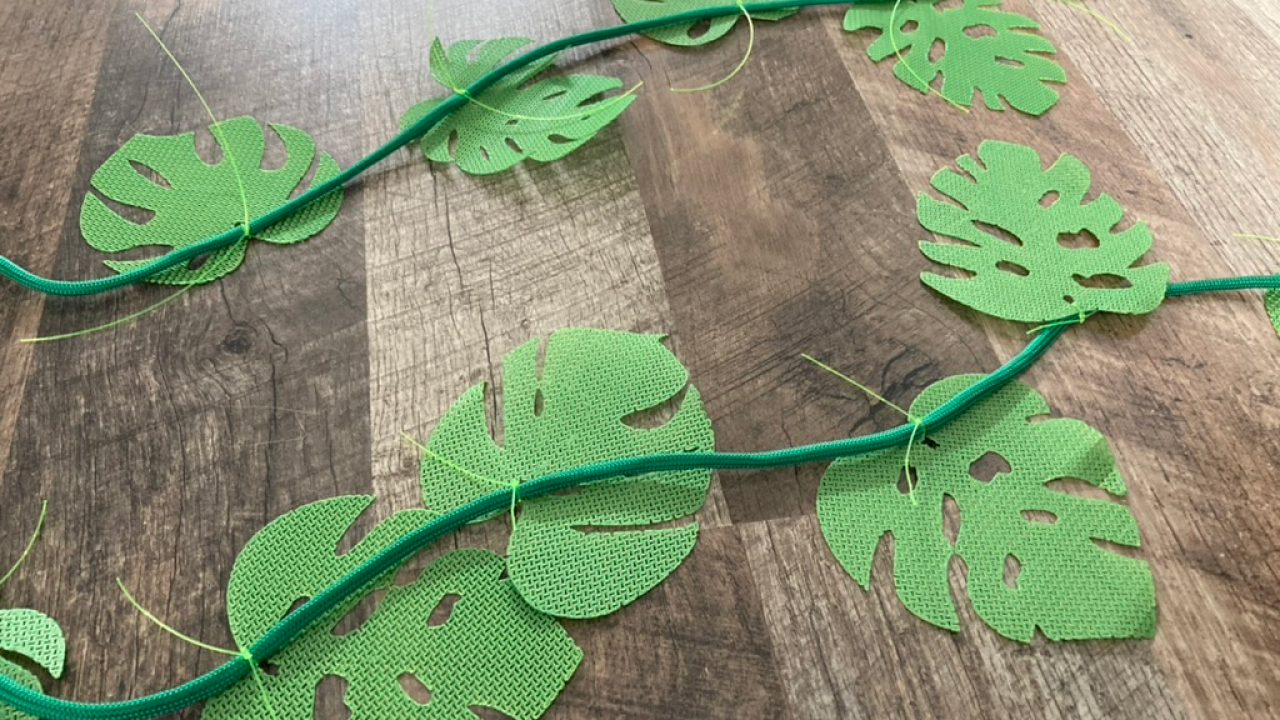
\includegraphics[width=\textwidth]{prototype_rope_leaves.jpg}
        \caption{Attaching the leaves with fishing line }
        \label{fig:attaching-leaves}
    \end{subfigure}
    \caption{Hanging planter strings attached to the paracord}
    \label{fig:prototype-leaves}
\end{figure}

\begin{figure}[htbp]
    \centering
    \begin{subfigure}{0.48\textwidth}
        \centering
        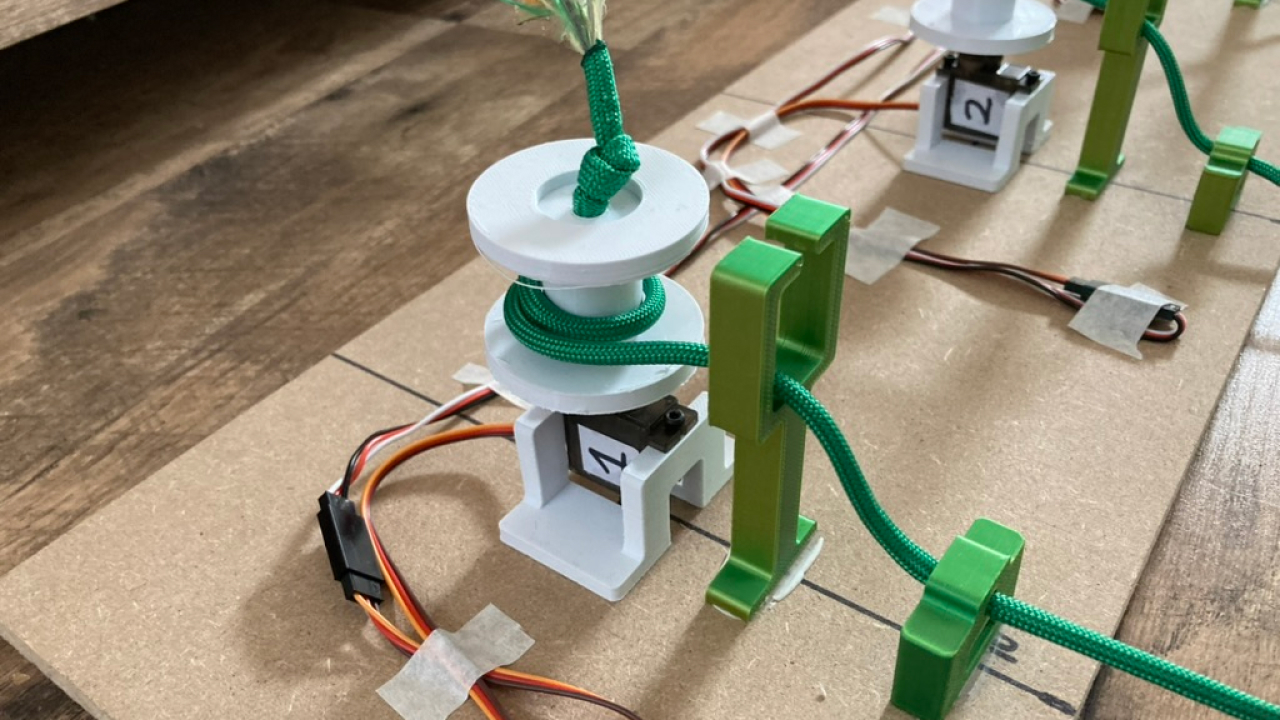
\includegraphics[width=\textwidth]{prototype_pulley_mechanism.jpg}
        \caption{Pulley mechanism installed with rope guides}
        \label{fig:pulley-small}
    \end{subfigure}
    \hfill
    \begin{subfigure}{0.48\textwidth}
        \centering
        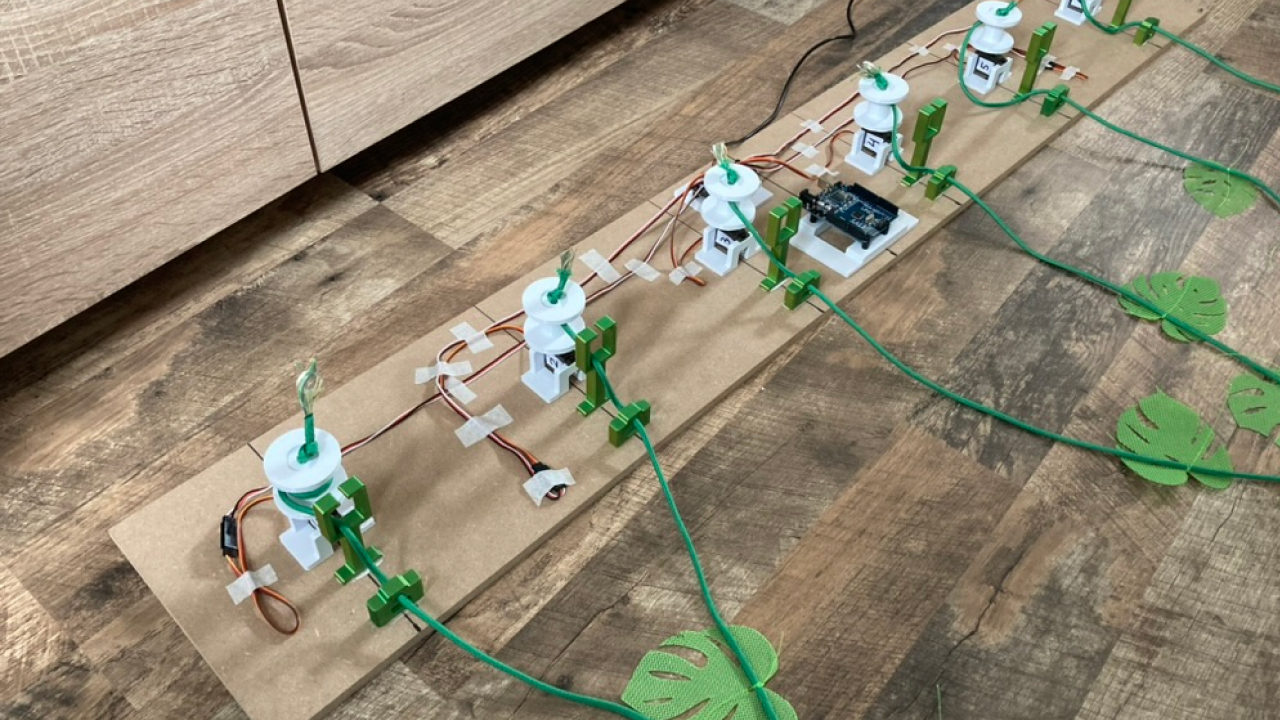
\includegraphics[width=\textwidth]{prototype_wooden_board.jpg}
        \caption{Attaching the electronics to the wooden board}
        \label{fig:pulley-large}
    \end{subfigure}
    \caption{Rear view of the prototype with all components mounted}
    \label{fig:prototype-board}
\end{figure}

\section{system architecture of the prototype}
\label{appendix:architecture}

System architecture diagram (see \hyperref[fig:system-diagram]{Figure \ref{fig:system-diagram}}) which shows the Internet of Things (IoT) architecture of the prototype following the notion of edge computing using a 1) sensing layer, 2) networking layer, 3) processing layer and 4) application layer.

\begin{figure}[H]
    \centering
    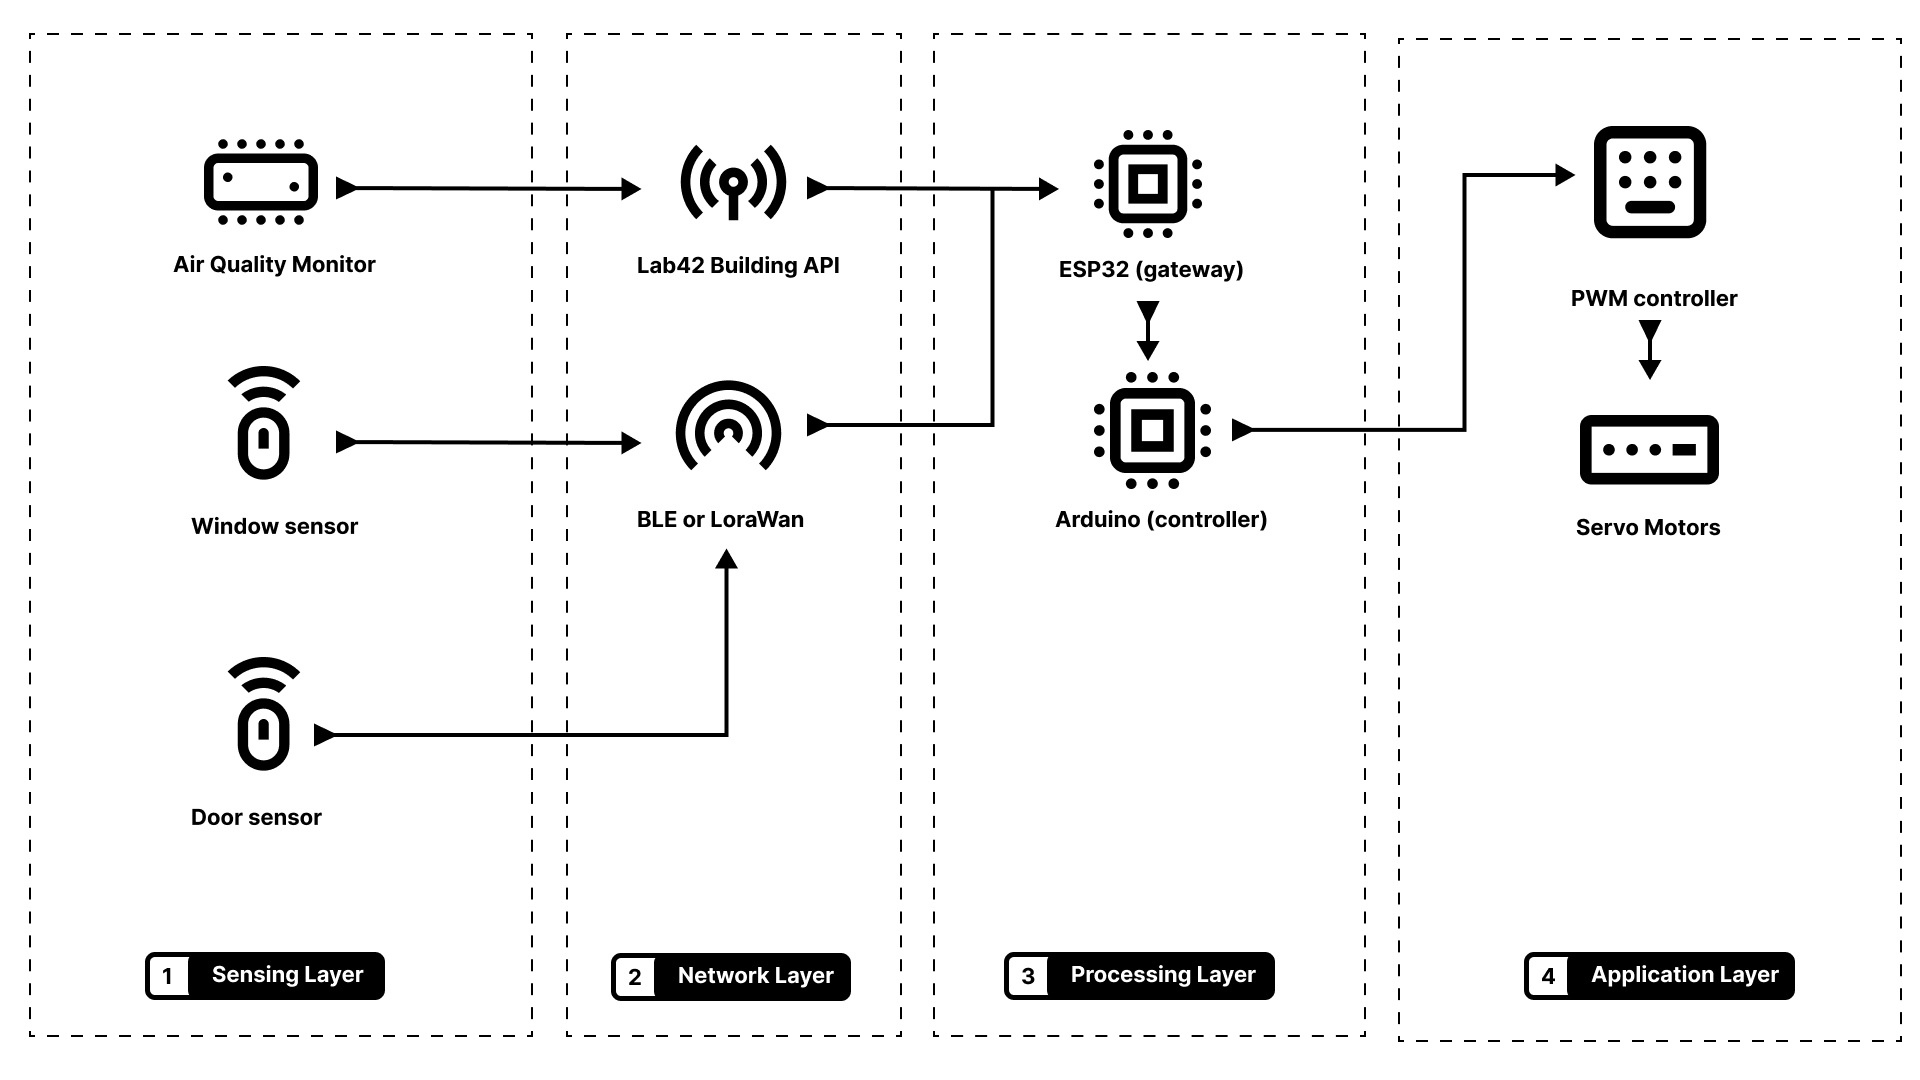
\includegraphics[width=0.65\paperwidth]{system_architecture.jpg}
    \caption{System diagram that shows the technical set-up of the prototype}
    \label{fig:system-diagram}
\end{figure}

\section{Lab42 API sample data}
\label{appendix:api-sample-data}

Screenshot of the internal Lab42 building API documentation (see \hyperref[fig:api-documentation]{Figure \ref{fig:api-documentation}}). The API offers access to reliable and detailed sensor data installed throughout the Lab42 building at Science Park. Designed as a research resource for university employees and students. The available sensors in a specific room can be gathered through a Room ID and data can be requested based on a specific date and timeframe.


\begin{figure}[H]
    \centering
    \begin{minipage}{0.7\textwidth}
        \centering
        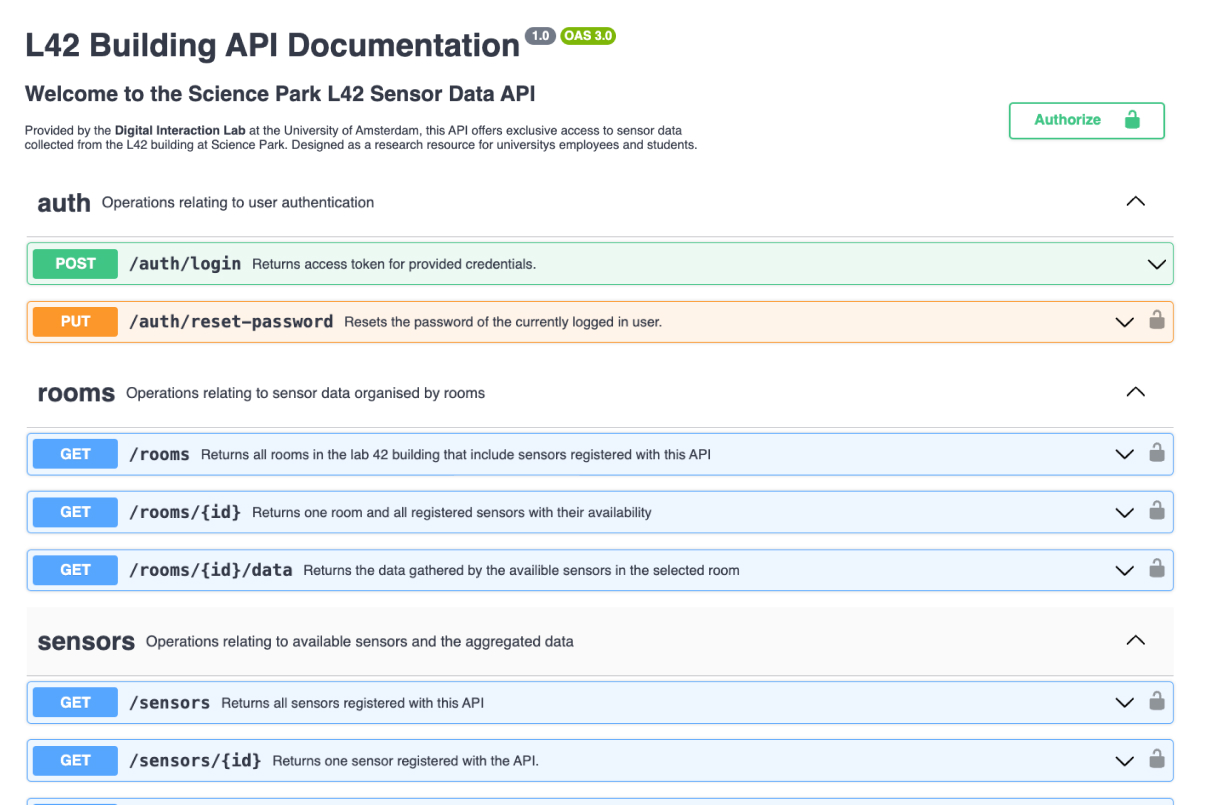
\includegraphics[width=\linewidth]{lab42_api.png}
    \end{minipage}%
    \begin{minipage}{0.3\textwidth}
        \centering
        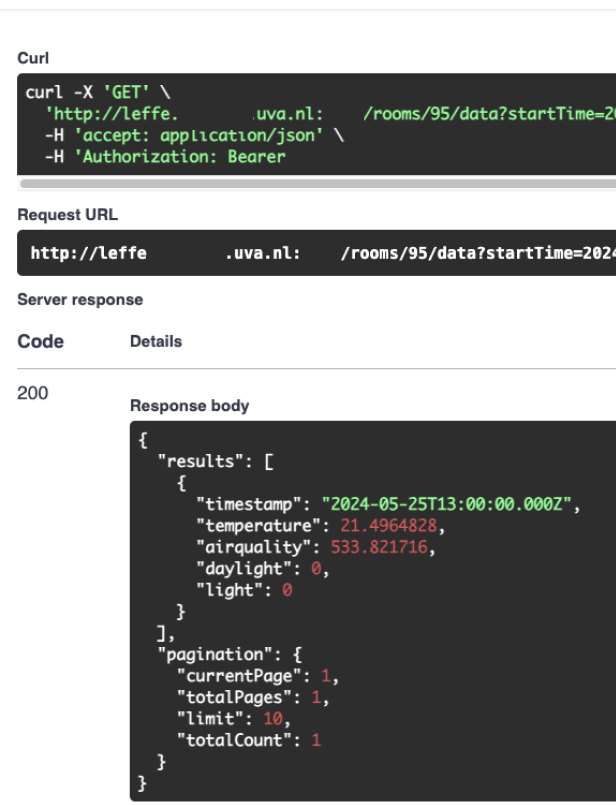
\includegraphics[width=\linewidth]{lab42_api_response.png}
    \end{minipage}
    \caption{Screenshot of the Lab42 building API documentation and sample data output log}
    \label{fig:api-documentation}
\end{figure}

\newpage

\section{Air Quality Monitors sample data}
\label{appendix:monitors}

Sample data logs (see \hyperref[tab:room-a]{Table \ref{tab:room-a}} and \hyperref[tab:room-b]{Table \ref{tab:room-b}} ) of the indoor air quality monitor devices installed in the small and large meeting rooms. These data logs were stored on-device during the data collection phase and exported for analysis. Both devices used the same polling rate but deferred in which sensory readings the device was capable of. Both have data and timestamps, CO2 concentrations, temperature and humidity which were used for the scope of this research.

\begin{table}[H]
    \centering
    \resizebox{\textwidth}{!}{%
    \tiny
    \begin{tabular}{@{} *{11}{c} @{}}
        \toprule
        \textbf{Date} & \textbf{Time} & \textbf{CO2} & \textbf{Temp} & \textbf{RH} & \textbf{PM1.0} & \textbf{PM2.5} & \textbf{PM10} & \textbf{TVOC} & \textbf{BP} & \textbf{O3} \\
        \midrule
        2024/04/03 & 10:30 & 647 & 21'C & 39\% & 0 & 0 & 0 & 255 & 99.97 & 0 \\
        2024/04/03 & 10:29 & 641 & 21'C & 39\% & 0 & 0 & 0 & 249 & 99.97 & 0 \\
        2024/04/03 & 10:28 & 633 & 21'C & 39\% & 0 & 0 & 0 & 246 & 99.97 & 0 \\
        2024/04/03 & 10:27 & 635 & 21'C & 39\% & 1 & 1 & 1 & 242 & 99.97 & 0 \\
        2024/04/03 & 10:26 & 632 & 21'C & 39\% & 0 & 1 & 1 & 237 & 99.97 & 0 \\
        2024/04/03 & 10:25 & 628 & 21'C & 39\% & 0 & 1 & 1 & 236 & 99.97 & 0 \\
        2024/04/03 & 10:24 & 617 & 21'C & 39\% & 0 & 1 & 1 & 232 & 99.97 & 0 \\
        2024/04/03 & 10:23 & 602 & 21'C & 39\% & 0 & 1 & 1 & 232 & 99.97 & 0 \\
        2024/04/03 & 10:22 & 598 & 21'C & 39\% & 0 & 0 & 0 & 231 & 99.97 & 0 \\
        2024/04/03 & 10:21 & 591 & 21'C & 39\% & 0 & 1 & 1 & 228 & 99.97 & 0 \\
        2024/04/03 & 10:20 & 587 & 21'C & 39\% & 0 & 0 & 0 & 228 & 99.97 & 0 \\
        2024/04/03 & 10:19 & 580 & 21'C & 39\% & 0 & 0 & 0 & 230 & 99.97 & 0 \\
        2024/04/03 & 10:18 & 580 & 21'C & 39\% & 0 & 0 & 0 & 232 & 99.97 & 0 \\
        \bottomrule
    \end{tabular}%
    }
    \vspace{10pt} 
    \caption{Sample data log of the Aircheq Touch Aero installed in the 'small' Room A} 
    \label{tab:room-a}
\end{table}

\begin{table}[H]
    \centering
    \resizebox{\textwidth}{!}{%
    \tiny
    \begin{tabular}{@{} *{11}{c} @{}}
        \toprule
        \textbf{Date} & \textbf{Time} & \textbf{Temp} & \textbf{RH} & \textbf{DewPoint} & \textbf{CO2} & \textbf{-} & \textbf{-} & \textbf{-} & \textbf{-} & \textbf{-} \\
        \midrule
        10/04/2024 & 14:17:00 & 21.019 & 30.780 & 3.176 & 871.000 \\
        10/04/2024 & 14:18:00 & 21.039 & 30.573 & 3.098 & 871.000 \\
        10/04/2024 & 14:19:00 & 21.019 & 30.365 & 2.985 & 827.000 \\
        10/04/2024 & 14:20:00 & 21.049 & 30.164 & 2.917 & 808.000 \\
        10/04/2024 & 14:21:00 & 21.059 & 29.895 & 2.838 & 808.000 \\
        10/04/2024 & 14:22:00 & 21.059 & 29.852 & 2.772 & 773.000 \\
        10/04/2024 & 14:23:00 & 21.059 & 29.730 & 2.723 & 773.000 \\
        10/04/2024 & 14:24:00 & 21.079 & 29.608 & 2.665 & 773.000 \\
        10/04/2024 & 14:25:00 & 21.059 & 29.486 & 2.607 & 721.000 \\
        10/04/2024 & 14:26:00 & 21.059 & 29.303 & 2.520 & 714.000 \\
        10/04/2024 & 14:27:00 & 21.049 & 29.242 & 2.482 & 714.000 \\
        10/04/2024 & 14:28:00 & 21.079 & 29.181 & 2.479 & 714.000 \\
        10/04/2024 & 14:29:00 & 21.059 & 29.016 & 2.400 & 681.000 \\
        10/04/2024 & 14:30:00 & 21.089 & 28.912 & 2.358 & 681.000 \\
        \bottomrule
    \end{tabular}%
    }\vspace{10pt} 
    \caption{Sample data log of the Atal ATU-CT ClimaTrend installed in the 'large' Room B} 
    \label{tab:room-b}
\end{table}


\section{Questionnaire survey (POE)}
\label{appendix:survey}

Exported text version of the questionnaire survey created in Qualtrics and distributed using handouts with QR codes.

\vspace{10pt} 

\textbf{Introduction:}
\textit{Hi! We at the Digital Interactions Lab (DIL) are researching indoor environments, focusing on Indoor Air Quality (IAQ) within smart buildings like Lab42, for a Master Thesis. This survey takes an average of $\sim$3 minutes to complete and comprises questions about your overall comfort and awareness of Indoor Air Quality (IAQ).}\\

\textbf{Informed Consent:}
\textit{The survey is anonymous and collects data on environmental experiences and approximate building location for future research and publication. Participation is voluntary, and if you decide that you do not want to participate after you have completed it, please contact us. Principal researcher: BSc D. de Vries - danny.de.vries@student.uva.nl Supervisor(s): Shruti Rao PhD Candidate - s.rao@uva.nl Supervisor(s): Dr. H. Seiied Alavi PhD - ha.alavi@uva.nl Thank you for your valuable time and for participating in our survey!}

\vspace{10pt} 

\textbf{Q1: Location}- Where are you currently located within the Lab42 building? \textit{Multiple-choice, one option possible}

\begin{itemize}
    \item On the ground floor (the atrium)
    \item On the first floor (1st floor - in a working space)
    \item On the second floor (2nd floor - in a working space)
\end{itemize}

\textbf{Q2: Activity} - On average, how often do you use Lab42 per week for various activities? \textit{Multiple-choice, one option possible}

\begin{itemize}
    \item 1 day a week
    \item 2 days a week
    \item 3 days a week
    \item 4 days a week
    \item 5 days a week
\end{itemize}

\textbf{Q3: Occupancy} - How would you describe the occupancy in your current space? \textit{Multiple-choice, one option possible}

\begin{itemize}
    \item Not crowded
    \item Not too crowded
    \item Crowded
    \item Very crowded
    \item At capacity
\end{itemize}

\textbf{Q4: Awareness Air Quality} - Did you know that poor air quality has been identified to pose health risks and affect cognitive performance? How aware are you of the current air quality in this space? \textit{Likert-scale, one option possible}

\textbf{1)} Very Unaware \textbf{2)} Unaware \textbf{3)} Neutral \textbf{4)} Aware \textbf{5)} Very Aware

\vspace{10pt}

\textbf{Q6: Perceived Air Quality} - How do you perceive the air quality in the current space? \textit{Likert-scale, one option possible}

\textbf{1)} Very Poor \textbf{2)} Poor \textbf{3)} Acceptable \textbf{4)} Good \textbf{5)} Very Good 

\vspace{10pt}

\textbf{Q7: Satisfaction Air Quality} - How satisfied are you with the air quality in the current space? \textit{Likert-scale, one option possible}

\textbf{1)} Very Dissatisfied \textbf{2)} Dissastisfied \textbf{3)} Neither dissatisfied or satisfied \textbf{4)} Satisfied \textbf{5)} Very Satisfied

\vspace{10pt}

\textbf{Q8: Not mandatory} - Would you like to describe in more detail in your own words how you currently feel about the Indoor Air Quality? \textit{Open-question, insert text}

\vspace{10pt}

\textbf{Q9: Health symptoms} - Do you experience any health-related symptoms based on the air quality in this space? \textit{Multiple-choice, multiple options possible, insert text field}

\begin{itemize}
    \item None
    \item Headaches
    \item Trouble breathing
    \item Feeling nauseating
    \item Other
\end{itemize}

\textbf{Q10: Cognitive symptoms} - Do you experience any cognitive-based symptoms on the air quality in this space? \textit{Multiple-choice, multiple options possible, insert text field}

\begin{itemize}
    \item None
    \item Trouble with focus
    \item Decreased productivity
    \item Tiredness
    \item Other
\end{itemize}


\section{Survey data}
\label{appendix:survey-data}

Plots for specific questions of the survey questionnaire data exported from Qualtrics. Bar charts are created to show the distribution of answers for each question (see \hyperref[fig:survey-bar-charts]{Figure \ref{fig:survey-bar-charts}}). The Likert scales are plotted as a stacked bar chart to show the scores (see \hyperref[fig:survey-stacked-Bars]{Figure \ref{fig:survey-stacked-bars}}).

\begin{figure}[htbp]
    \centering
    \begin{subfigure}{0.4\textwidth}
        \centering
        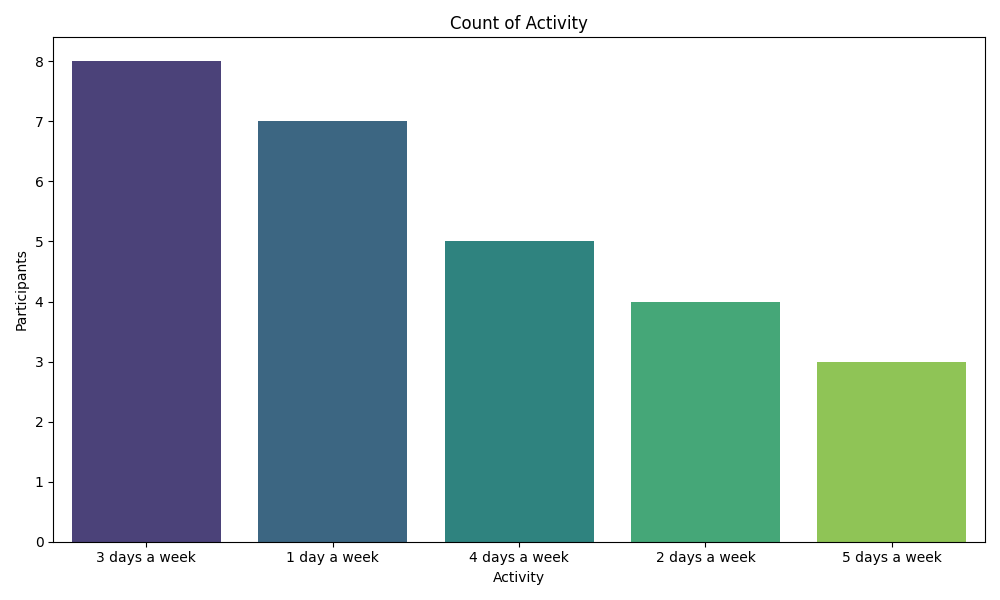
\includegraphics[width=\textwidth]{activity_bar_chart.png}
        \caption{Average use of the building for various activities}
        \label{fig:survey_building}
    \end{subfigure}
    \hfill
    \begin{subfigure}{0.4\textwidth}
        \centering
        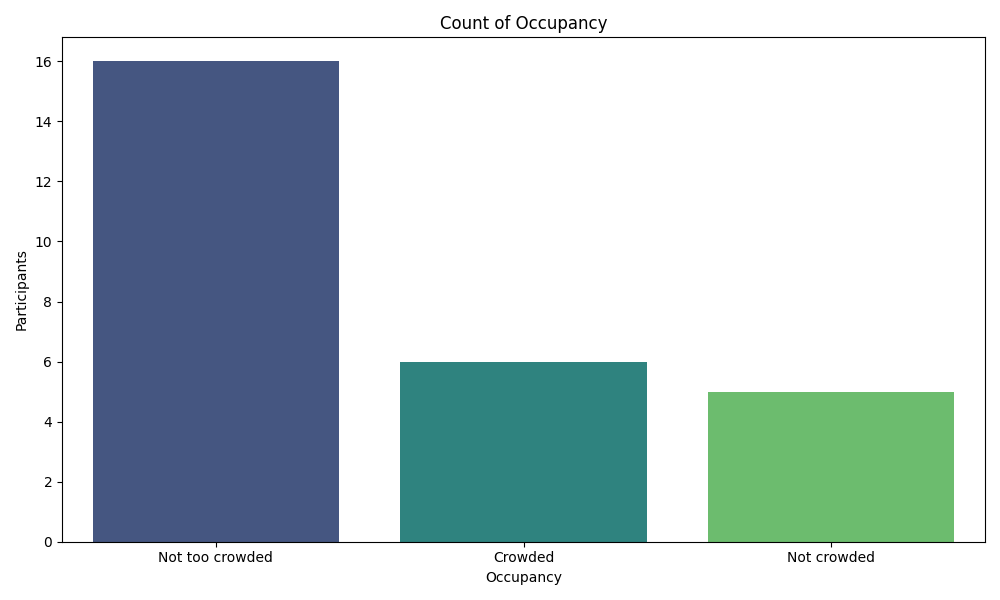
\includegraphics[width=\textwidth]{occupancy_bar_chart.png}
        \caption{Description of occupancy crowdedness}
        \label{fig:survey-occupancy}
    \end{subfigure}
    \begin{subfigure}{0.4\textwidth}
        \centering
        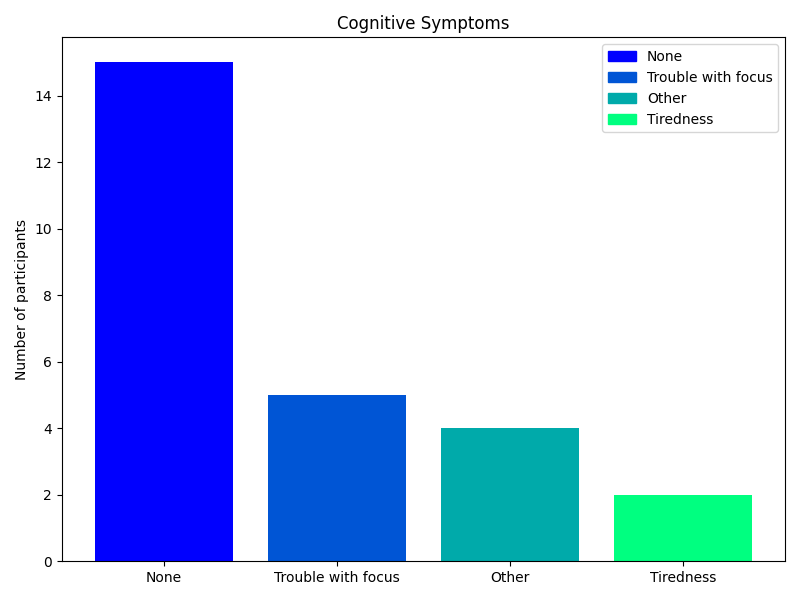
\includegraphics[width=\textwidth]{cognitive_symptomps.png}
        \caption{Cognitive symptoms based on the air quality}
        \label{fig:survey-cognitive}
    \end{subfigure}
    \hfill
    \begin{subfigure}{0.4\textwidth}
        \centering
        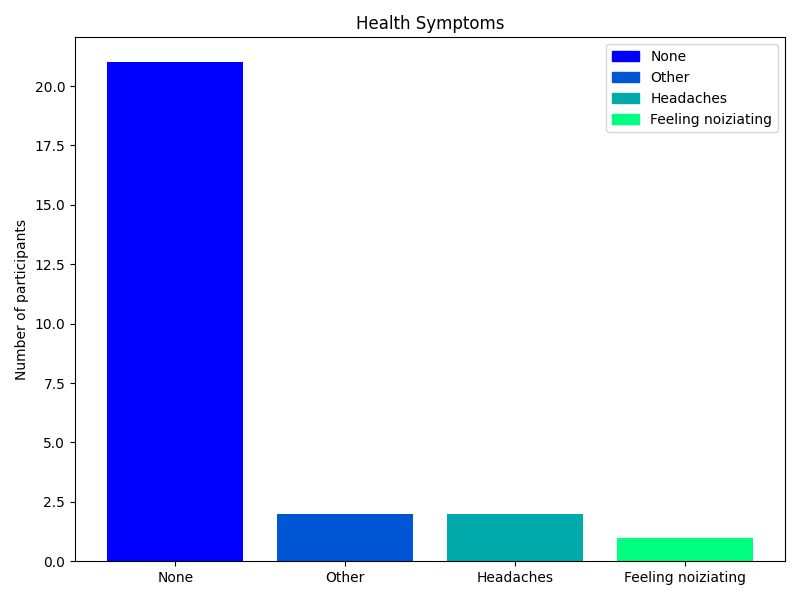
\includegraphics[width=\textwidth]{health_symptomps.png}
        \caption{Health symptoms based on the air quality}
        \label{fig:survey-health}
    \end{subfigure}    
    \caption{Bar charts of the survey questions about activity, occupancy, health and cognitive symptoms}
    \label{fig:survey-bar-charts}
\end{figure}

\begin{figure}[htbp]
    \centering
    \begin{subfigure}{0.18\textwidth}
        \centering
        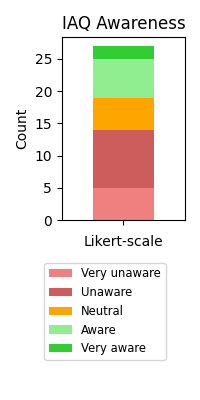
\includegraphics[width=\textwidth]{iaq_awareness.png}
        \caption{IAQ Awareness}
        \label{fig:survey-awareness}
    \end{subfigure}
    \hfill
    \begin{subfigure}{0.18\textwidth}
        \centering
        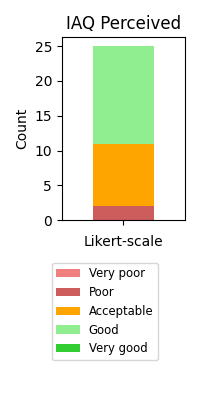
\includegraphics[width=\textwidth]{iaq_perceived.png}
        \caption{IAQ Perceived}
        \label{fig:survey-perceived}
    \end{subfigure}
    \hfill
    \begin{subfigure}{0.18\textwidth}
        \centering
        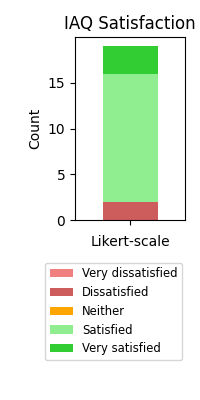
\includegraphics[width=\textwidth]{iaq_satisfaction.png}
        \caption{IAQ Satisfaction}
        \label{fig:survey-satisfaction}
    \end{subfigure}    
    \caption{Stacked bar charts of the Likert-scales on IAQ awareness, perceived and satisfaction}
    \label{fig:survey-stacked-bars}
\end{figure}

\newpage

\section{Monitor data}
\label{appendix:monitor-data}

Plots of the indoor air quality monitor data logs (see \hyperref[fig:monitoring-single]{Figure \ref{fig:monitoring-single}}, \hyperref[fig:monitoring-multiple]{Figure \ref{fig:monitoring-multiple}}, \hyperref[fig:monitoring-heatmap]{Figure \ref{fig:monitoring-heatmap}}). All graphs show the CO2 concentrations in either the small (Room A) or large (Room B) meeting rooms. The plots are subsets of the data logs which show interesting patterns and peaks based on the observed timeframe of the data collection phase.

\begin{figure}[htbp]
    \centering
    \begin{subfigure}{0.46\textwidth}
        \centering
        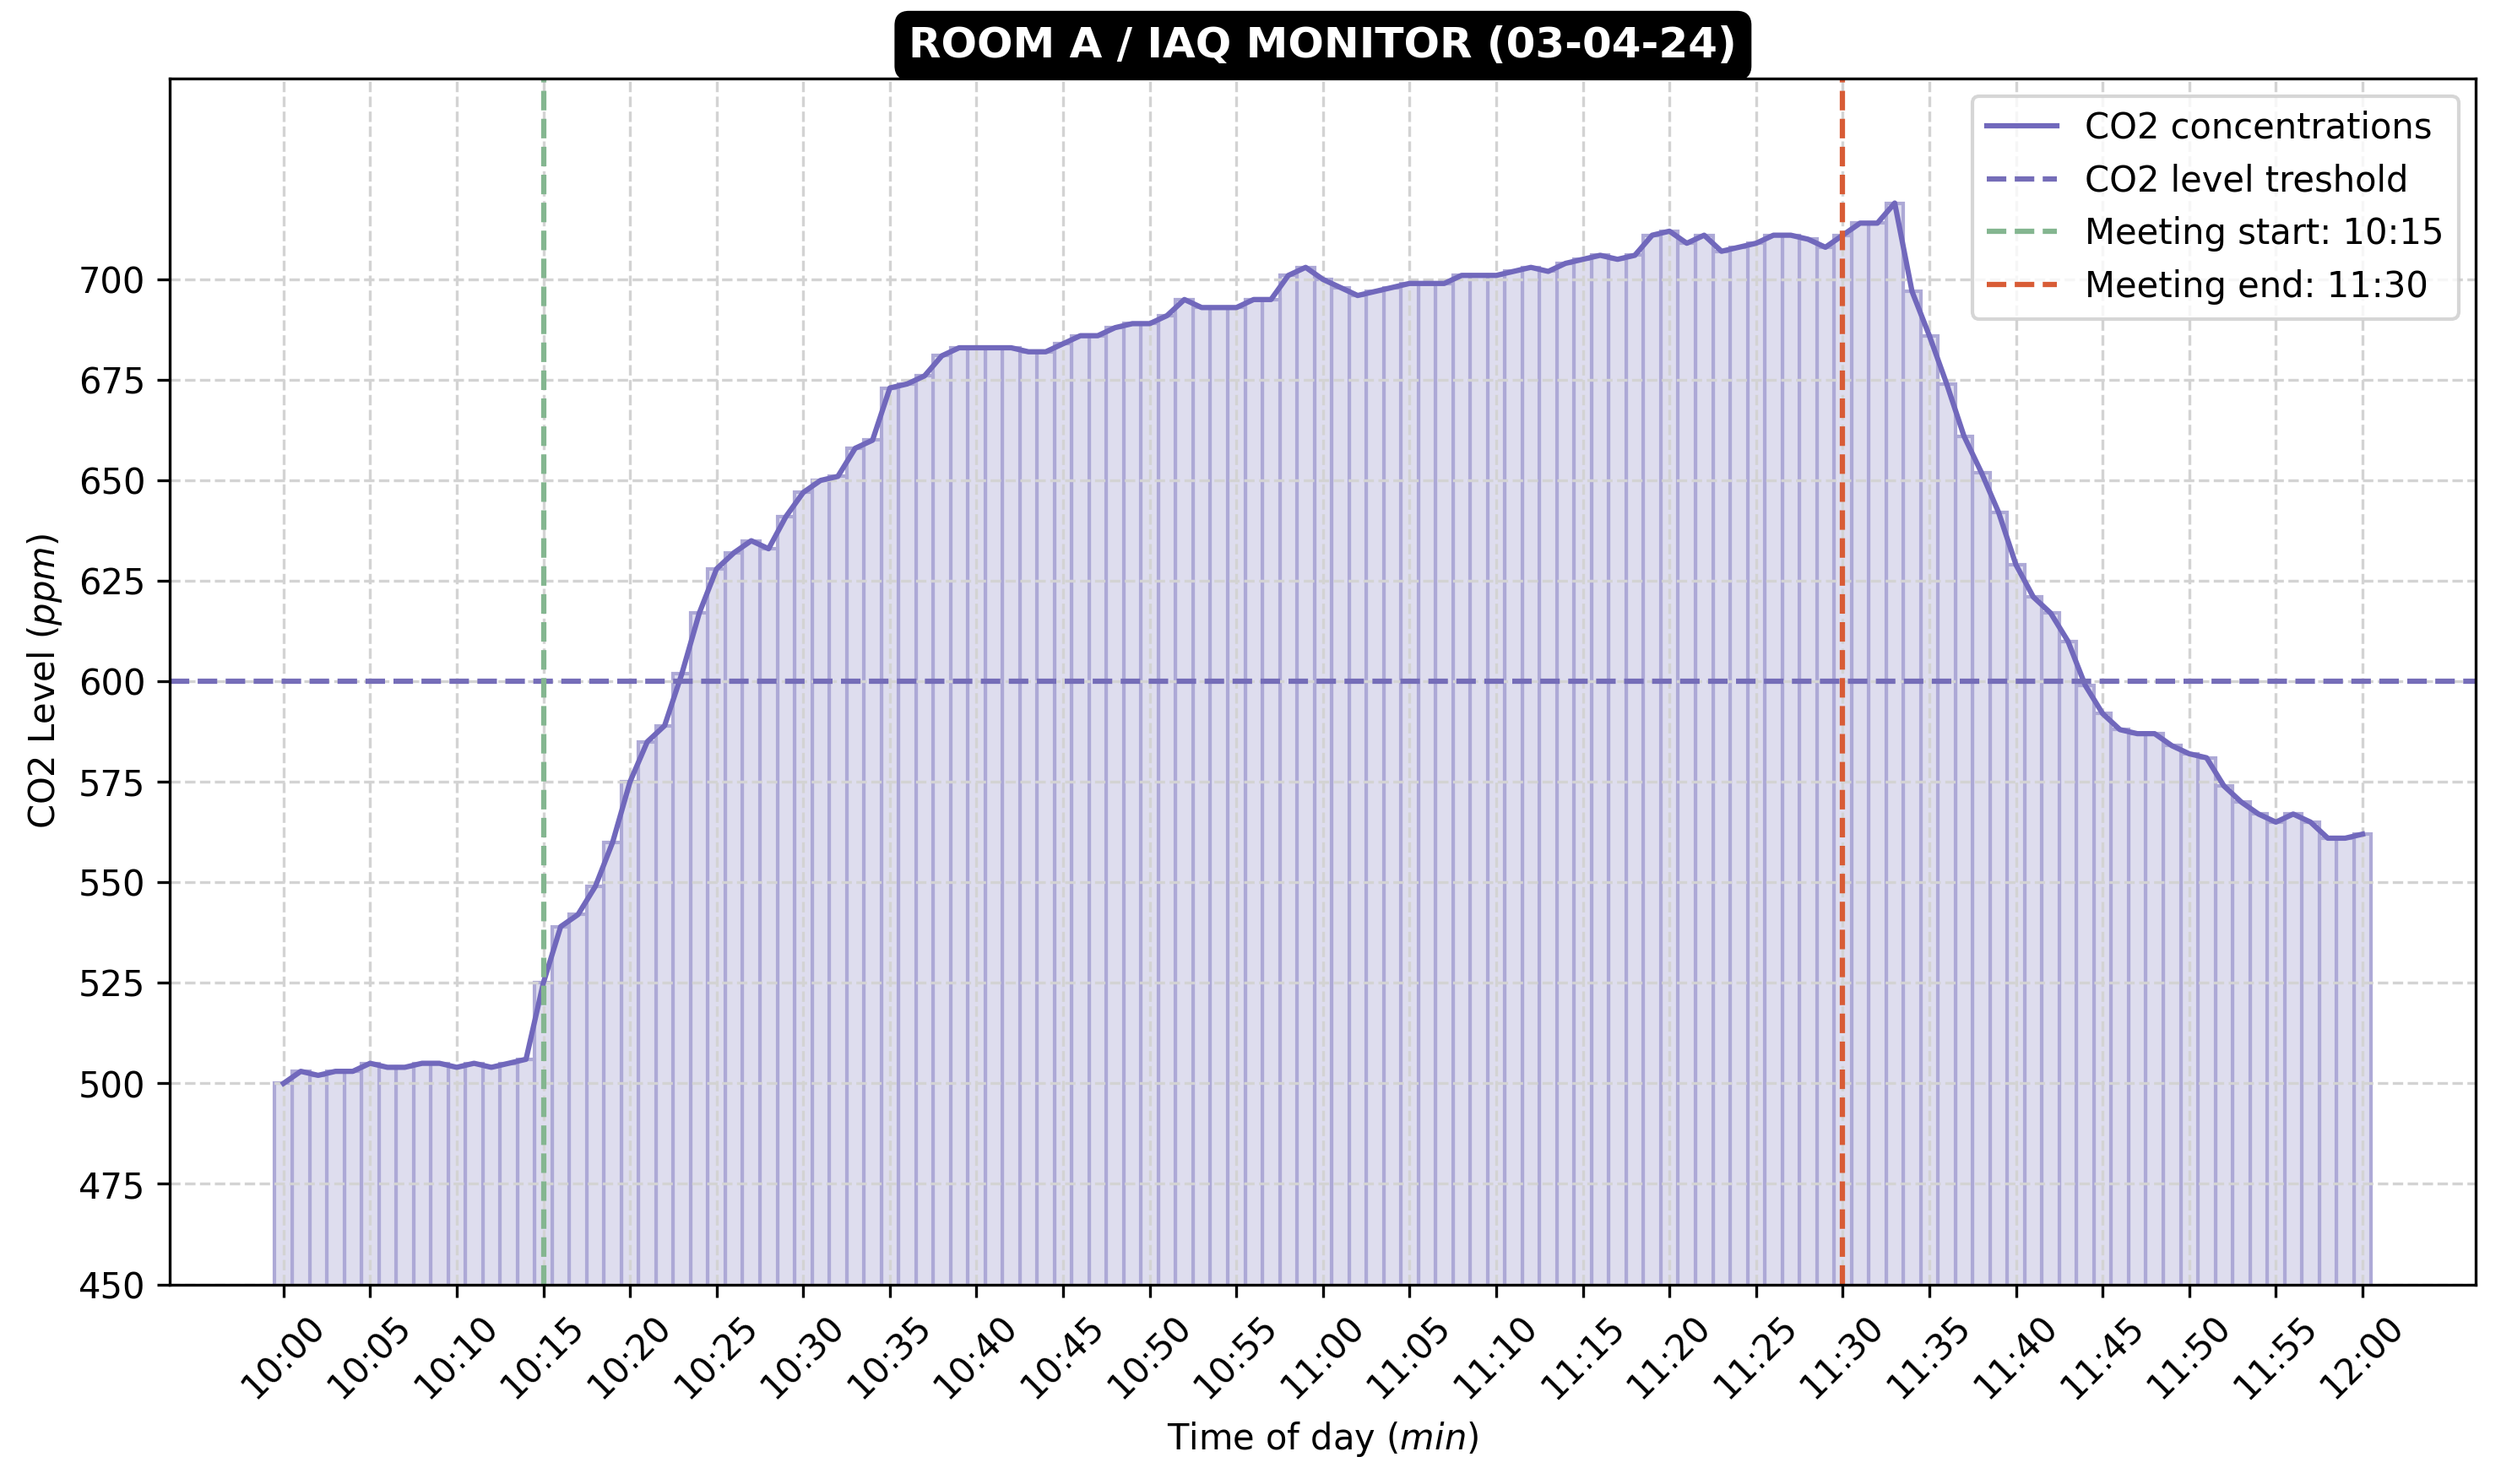
\includegraphics[width=\textwidth]{room-a-monitor-meeting-spike-single.png}
        \caption{Single meeting CO2 concentrations in Room A}
        \label{fig:monitor-single-a}
    \end{subfigure}
    \hfill
    \begin{subfigure}{0.46\textwidth}
        \centering
        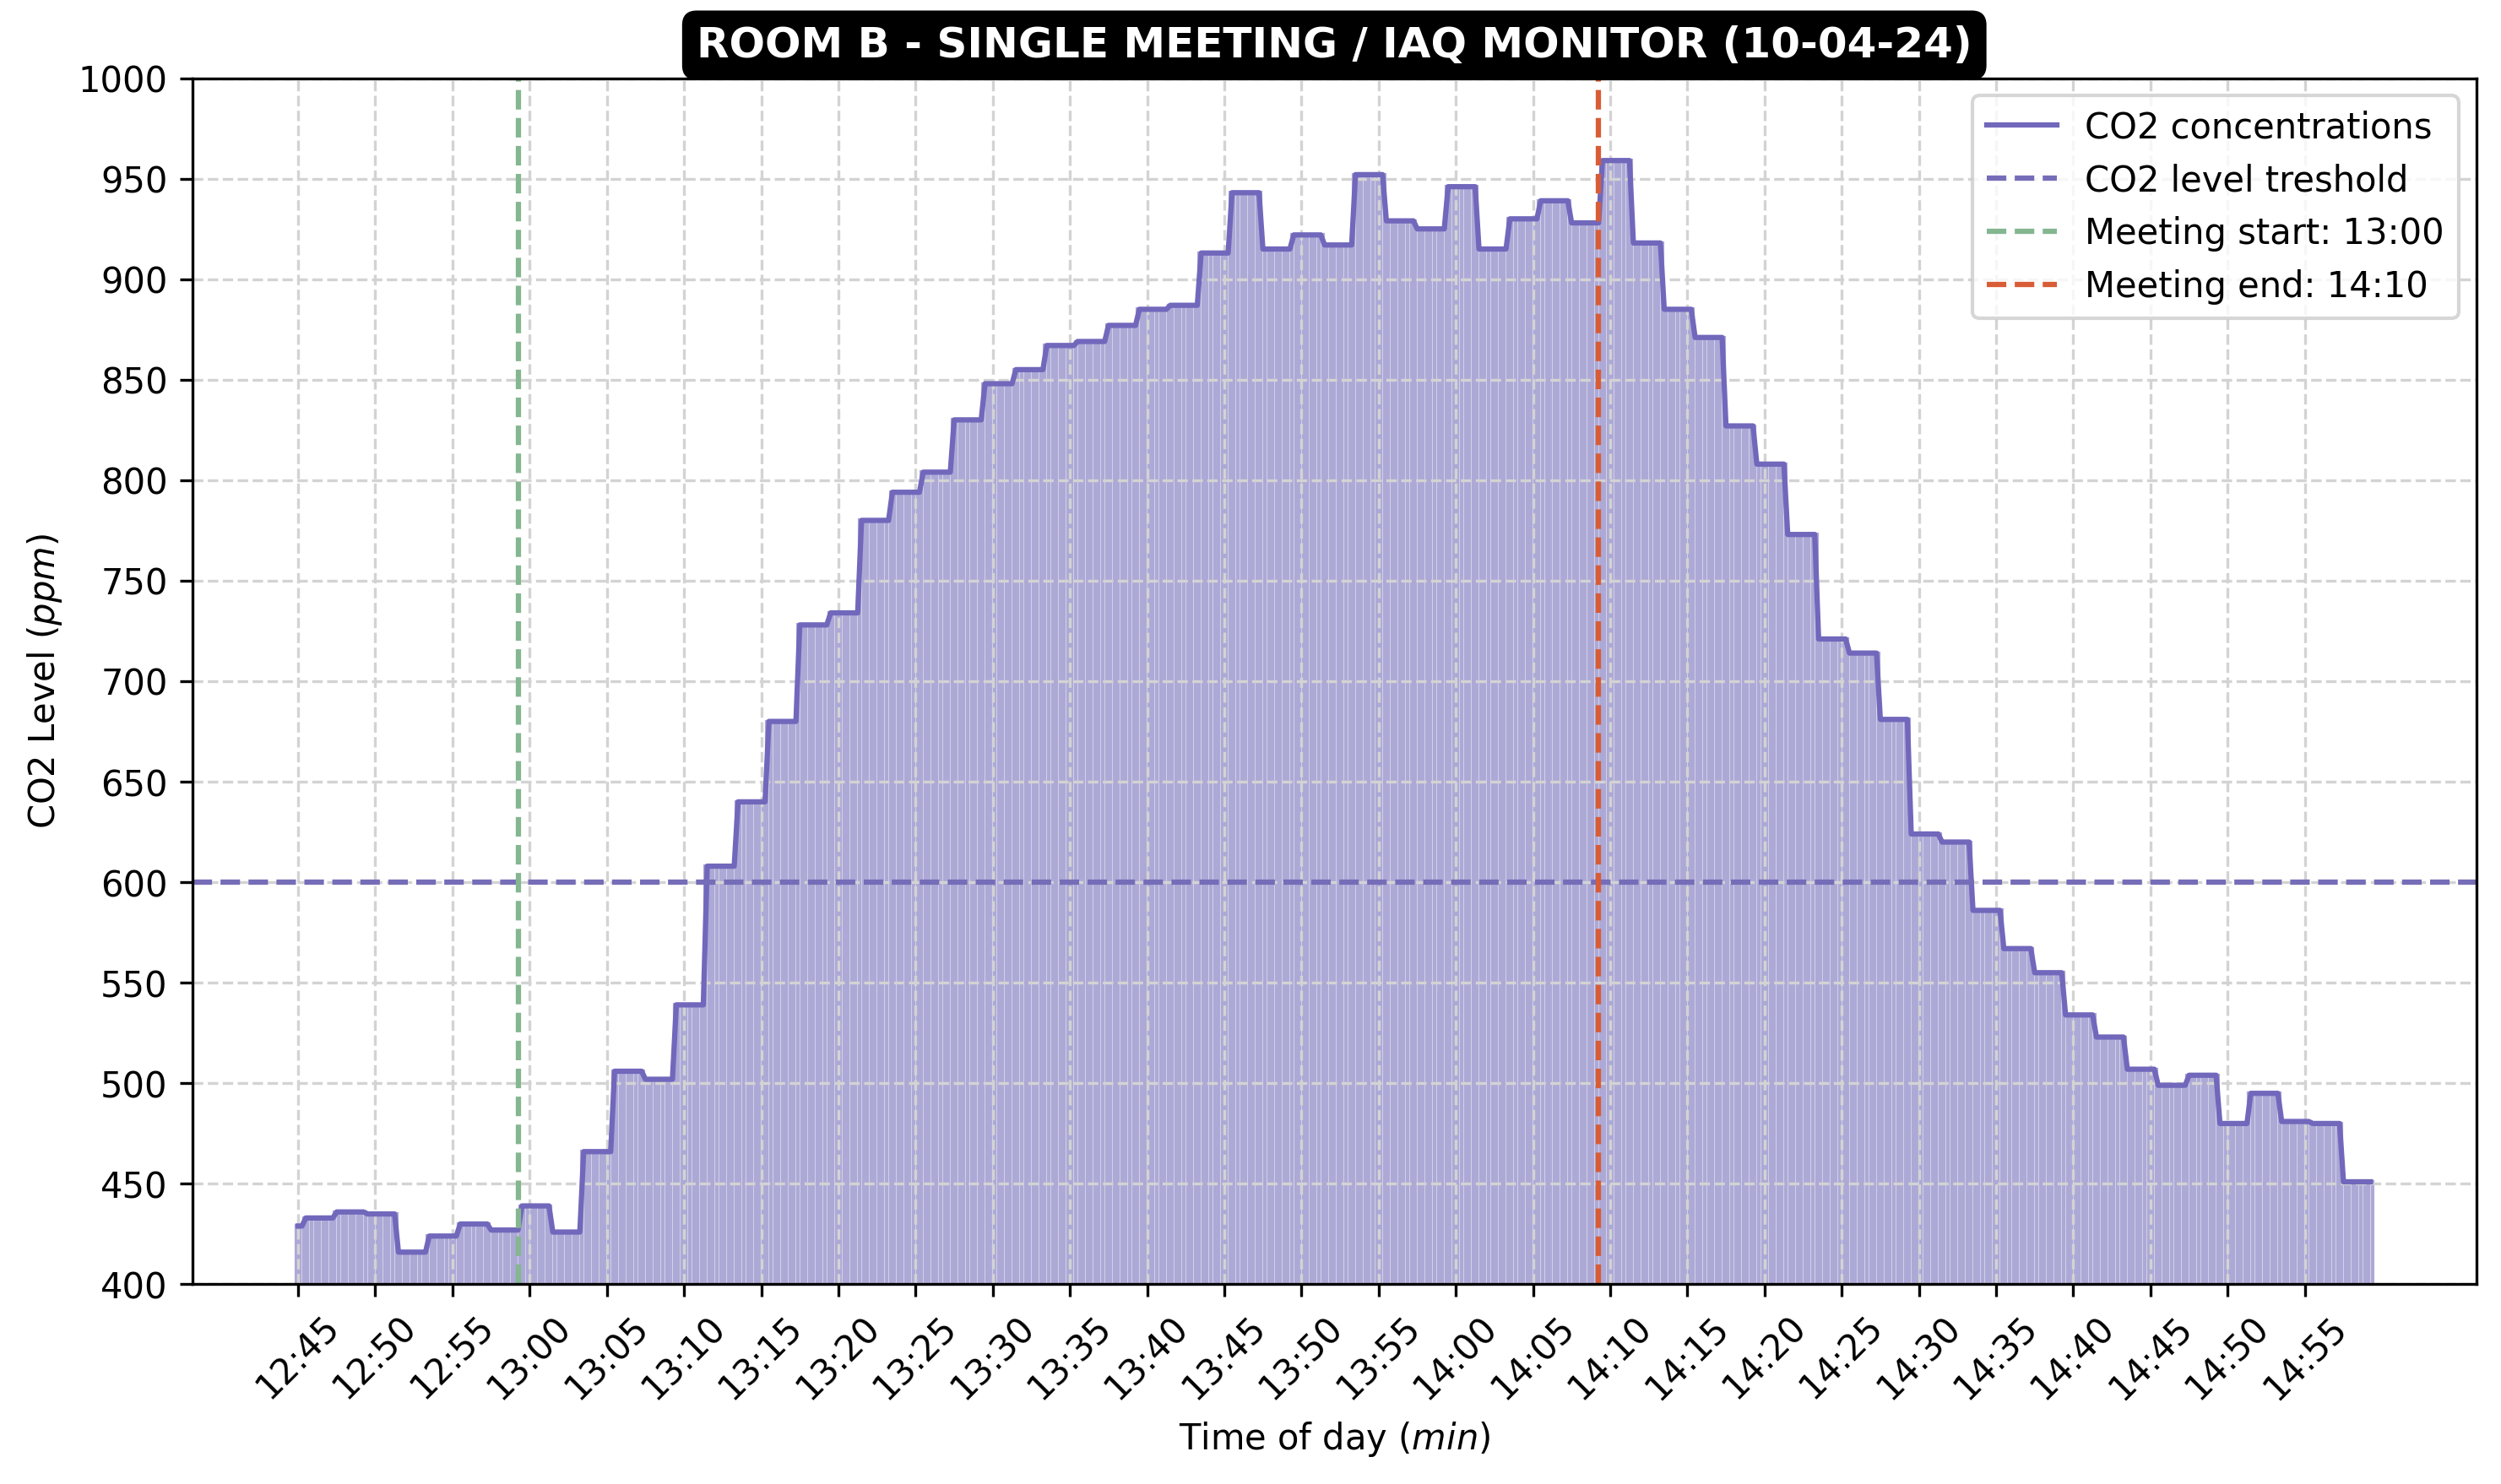
\includegraphics[width=\textwidth]{room-b-monitor-meeting-spike-single.png}
        \caption{Single meeting CO2 concentrations in Room B}
        \label{fig:monitor-single-b}
    \end{subfigure}
    \caption{IAQ monitoring CO2 concentrations of a single sample meeting based on the start and end time of the meeting}
    \label{fig:monitoring-single}
\end{figure}

\begin{figure}[htbp]
    \centering
    \begin{subfigure}{0.46\textwidth}
        \centering
        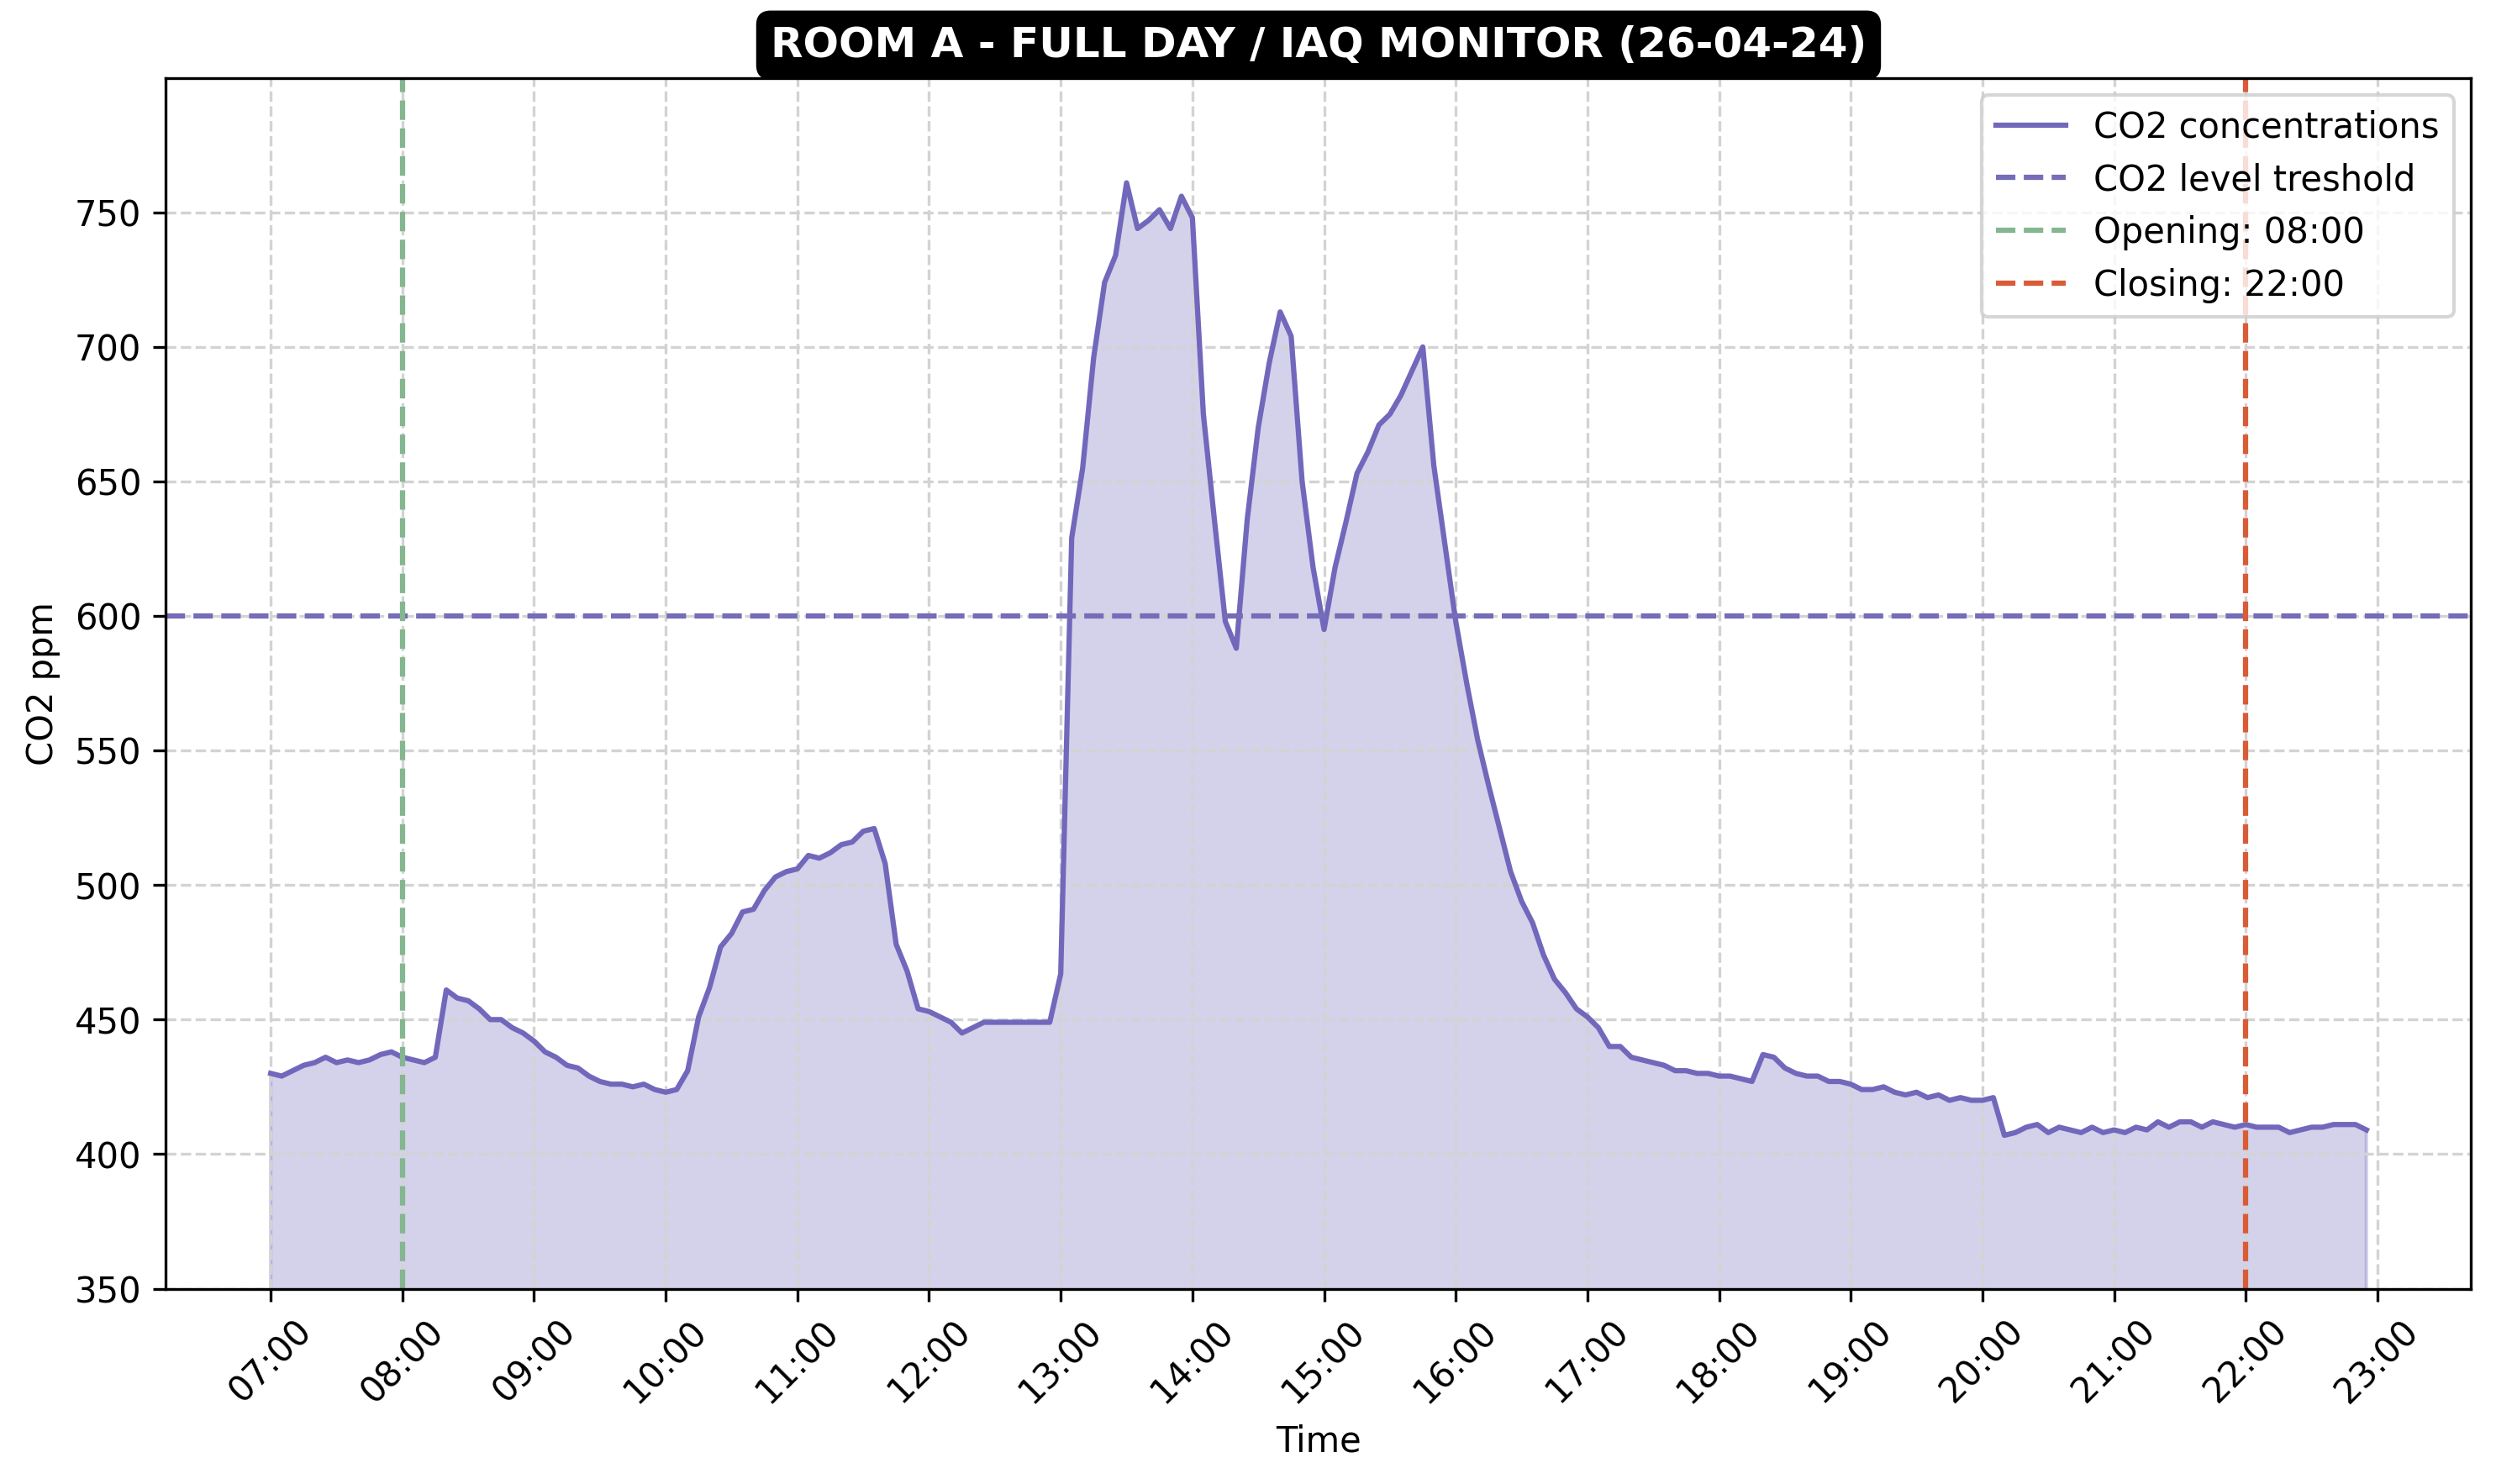
\includegraphics[width=\textwidth]{room-a-monitor-meeting-spike-day.png}
        \caption{A day of meetings CO2 concentrations in Room A}
        \label{fig:monitor-multiple-a}
    \end{subfigure}
    \hfill
    \begin{subfigure}{0.46\textwidth}
        \centering
        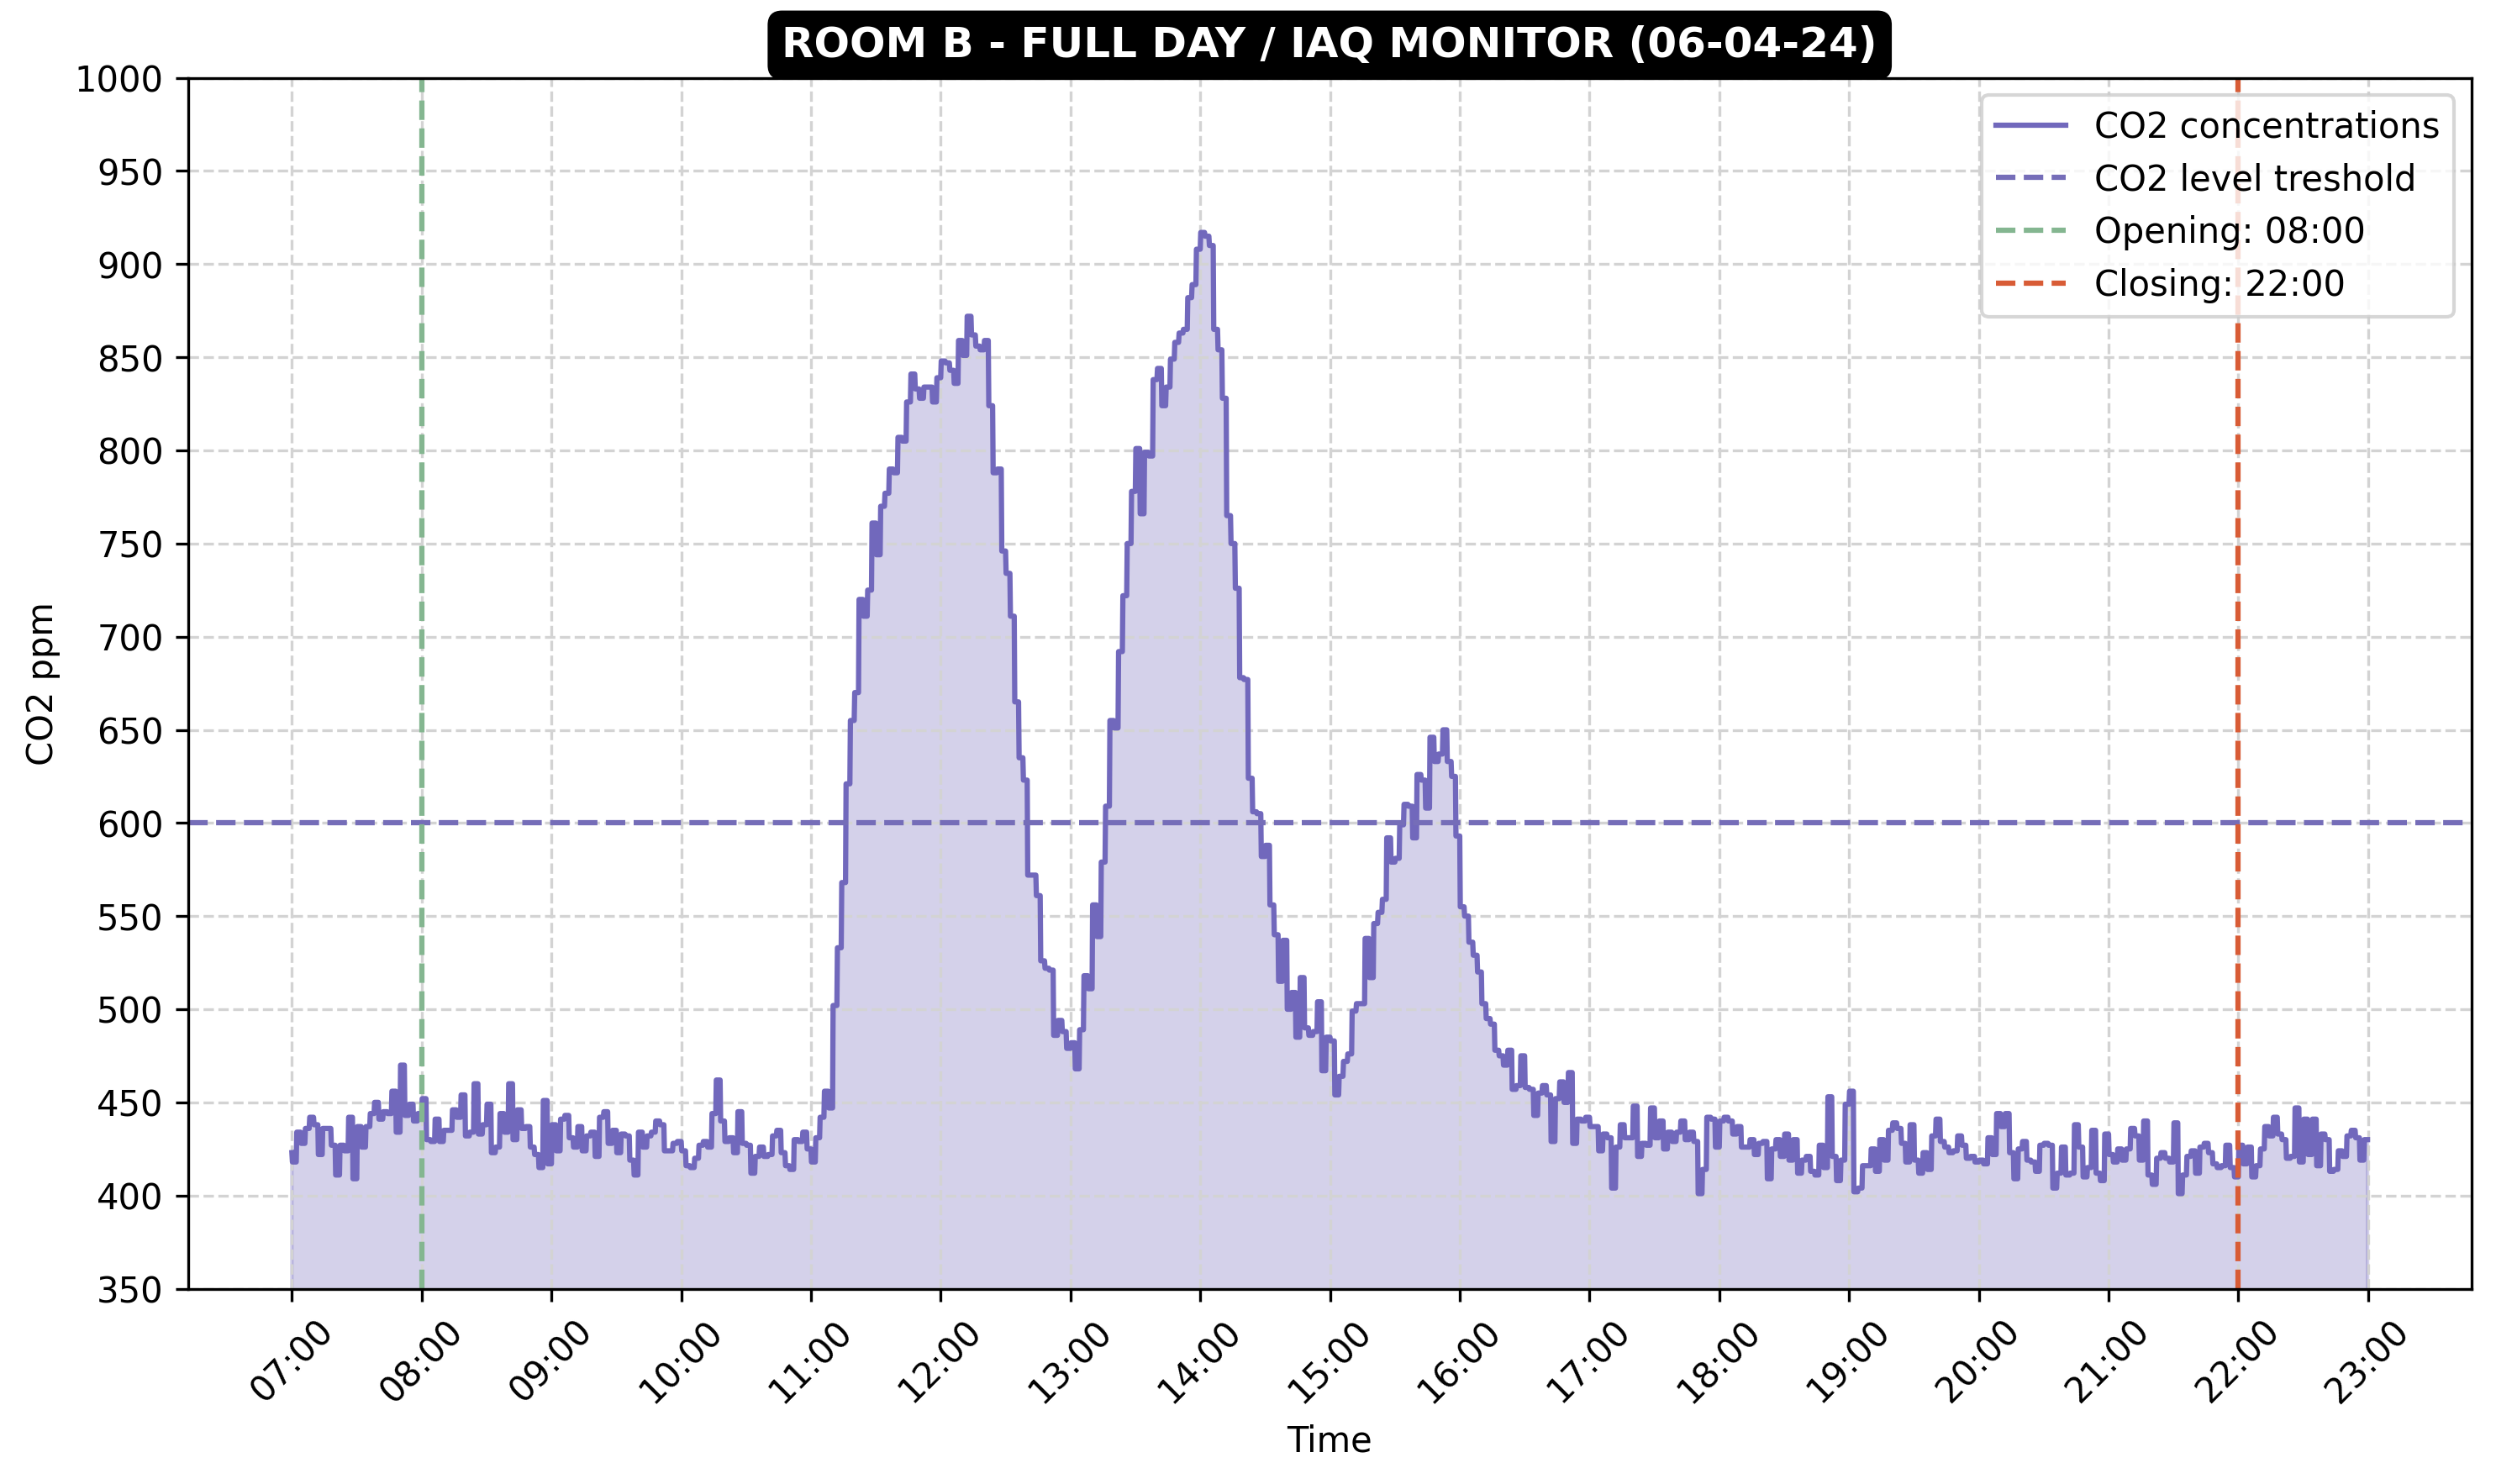
\includegraphics[width=\textwidth]{room-b-monitor-meeting-spike-day.png}
        \caption{A day of meetings CO2 concentrations in Room B}
        \label{fig:monitor-multiple-b}
    \end{subfigure}
    \caption{IAQ monitoring CO2 concentrations of a sample day meeting based on the opening hours of the building}
    \label{fig:monitoring-multiple}
\end{figure}

\begin{figure}[htbp]
    \centering
    \begin{subfigure}{0.46\textwidth}
        \centering
        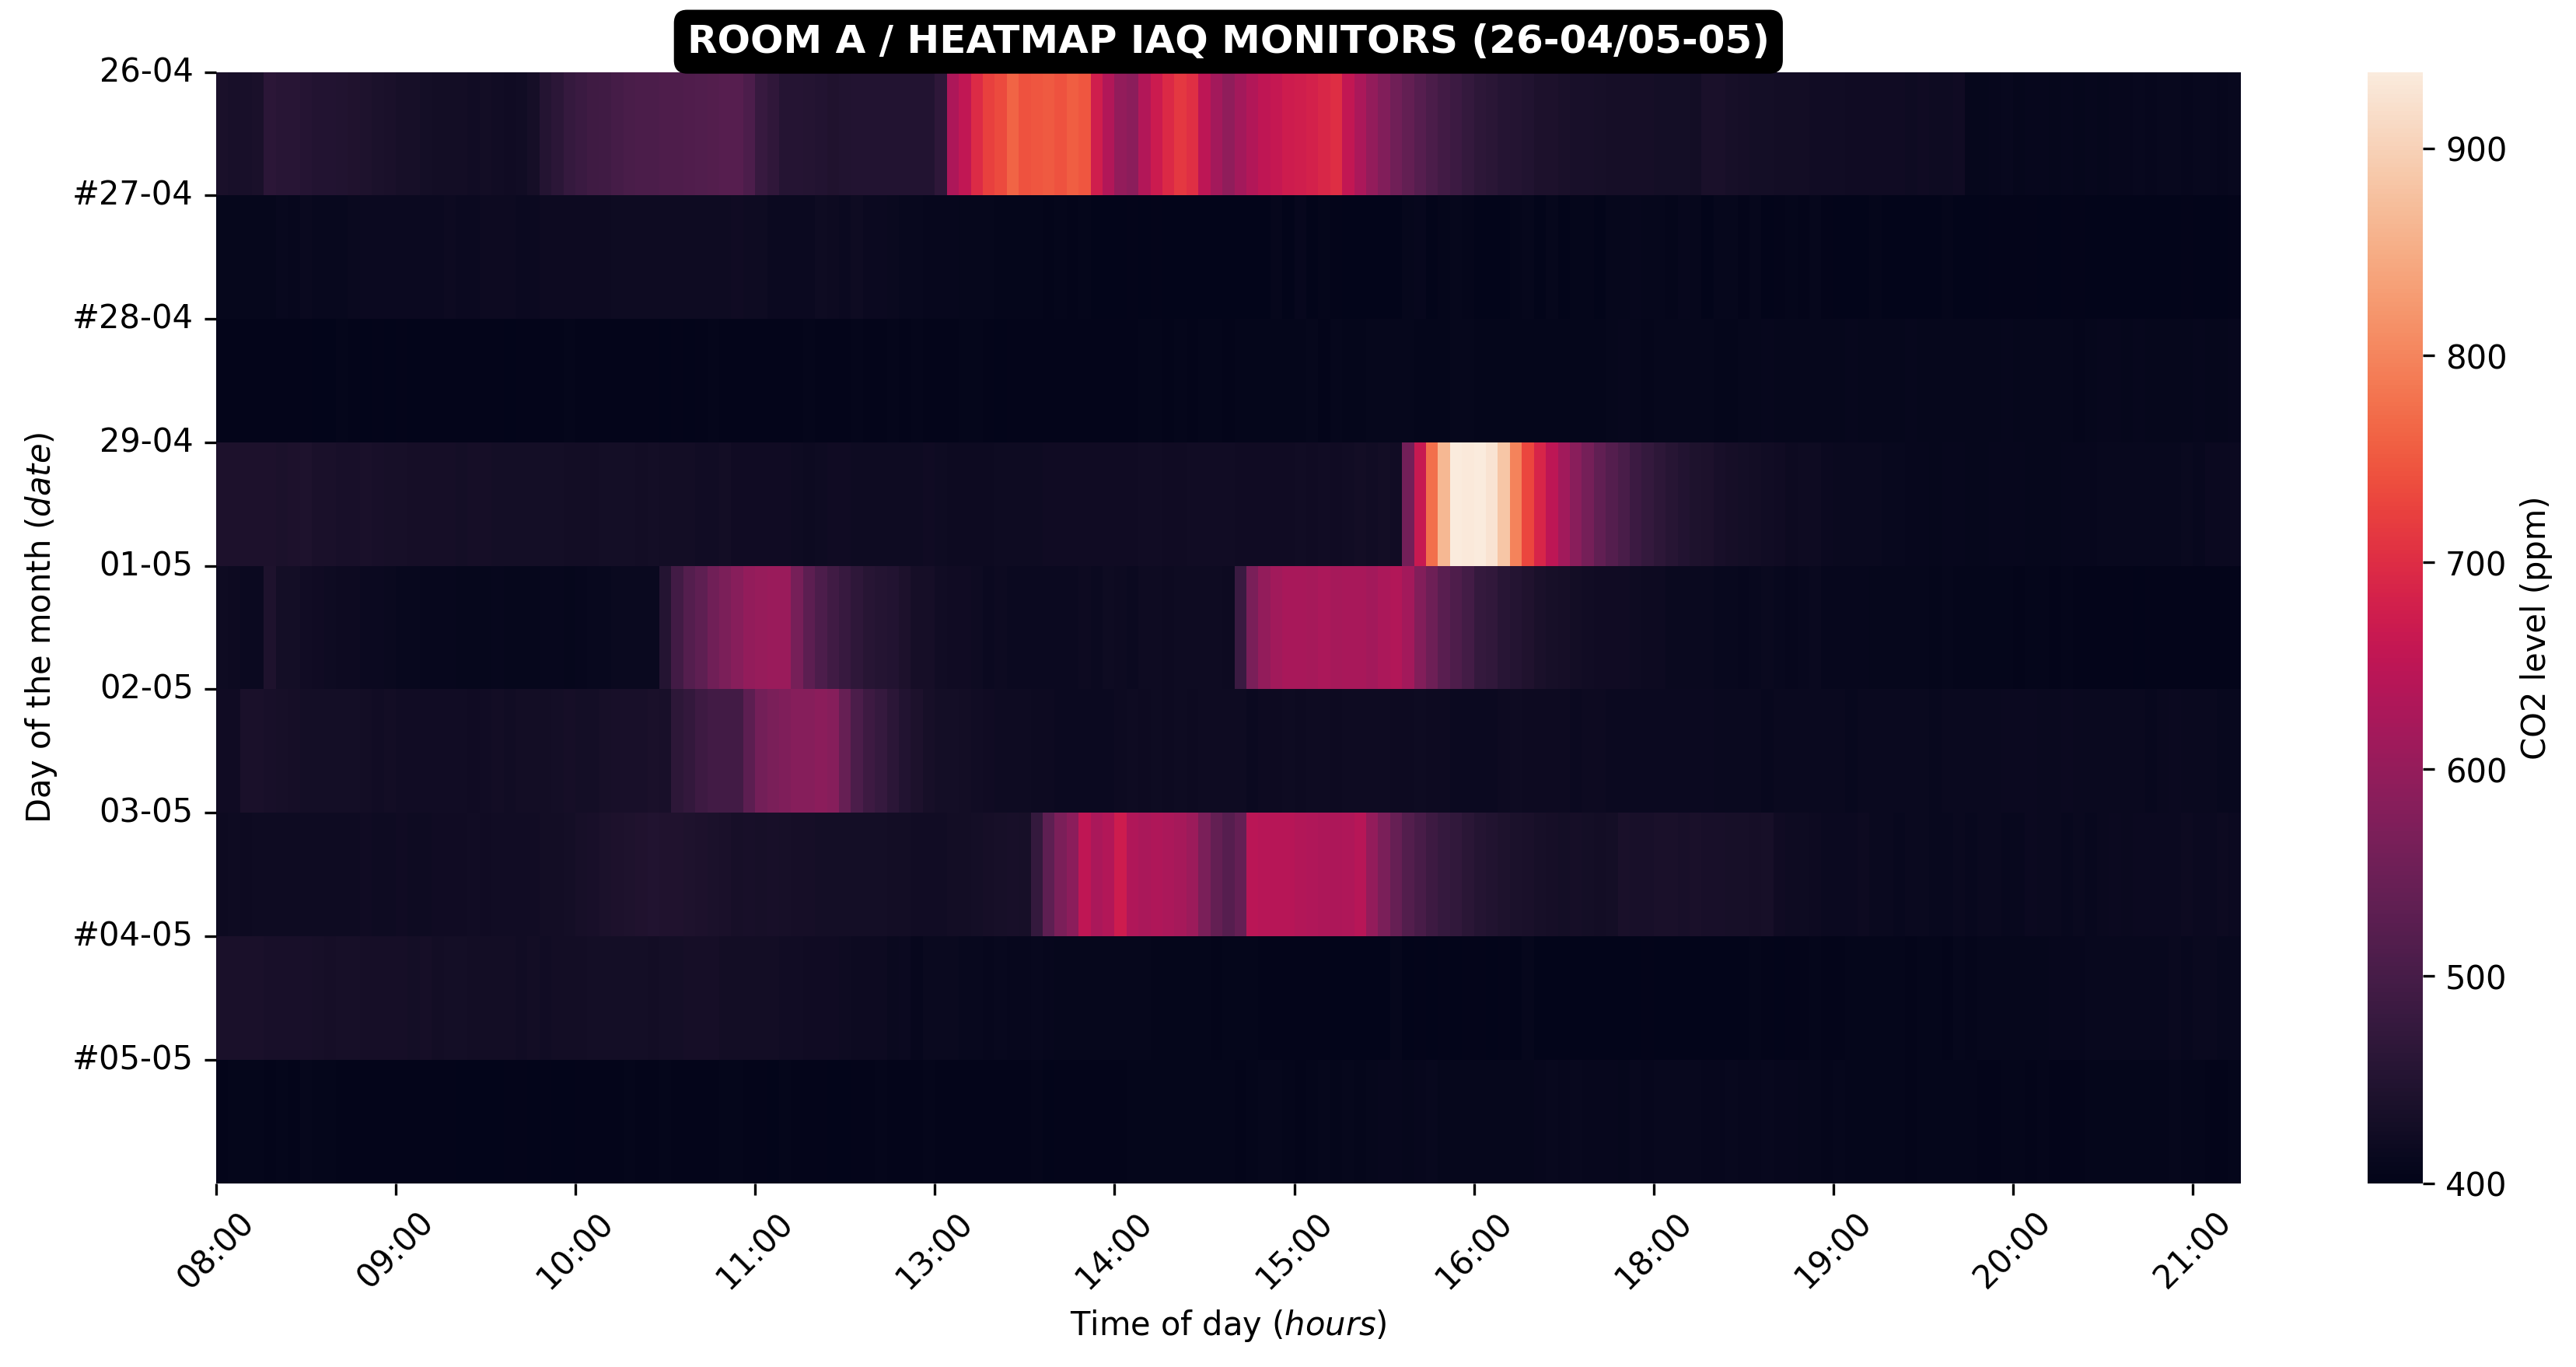
\includegraphics[width=\textwidth]{room-a-monitor-heatmap.png}
        \caption{Heatmap of ten days of monitoring in Room A}
        \label{fig:monitor-heatmap-a}
    \end{subfigure}
    \hfill
    \begin{subfigure}{0.46\textwidth}
        \centering
        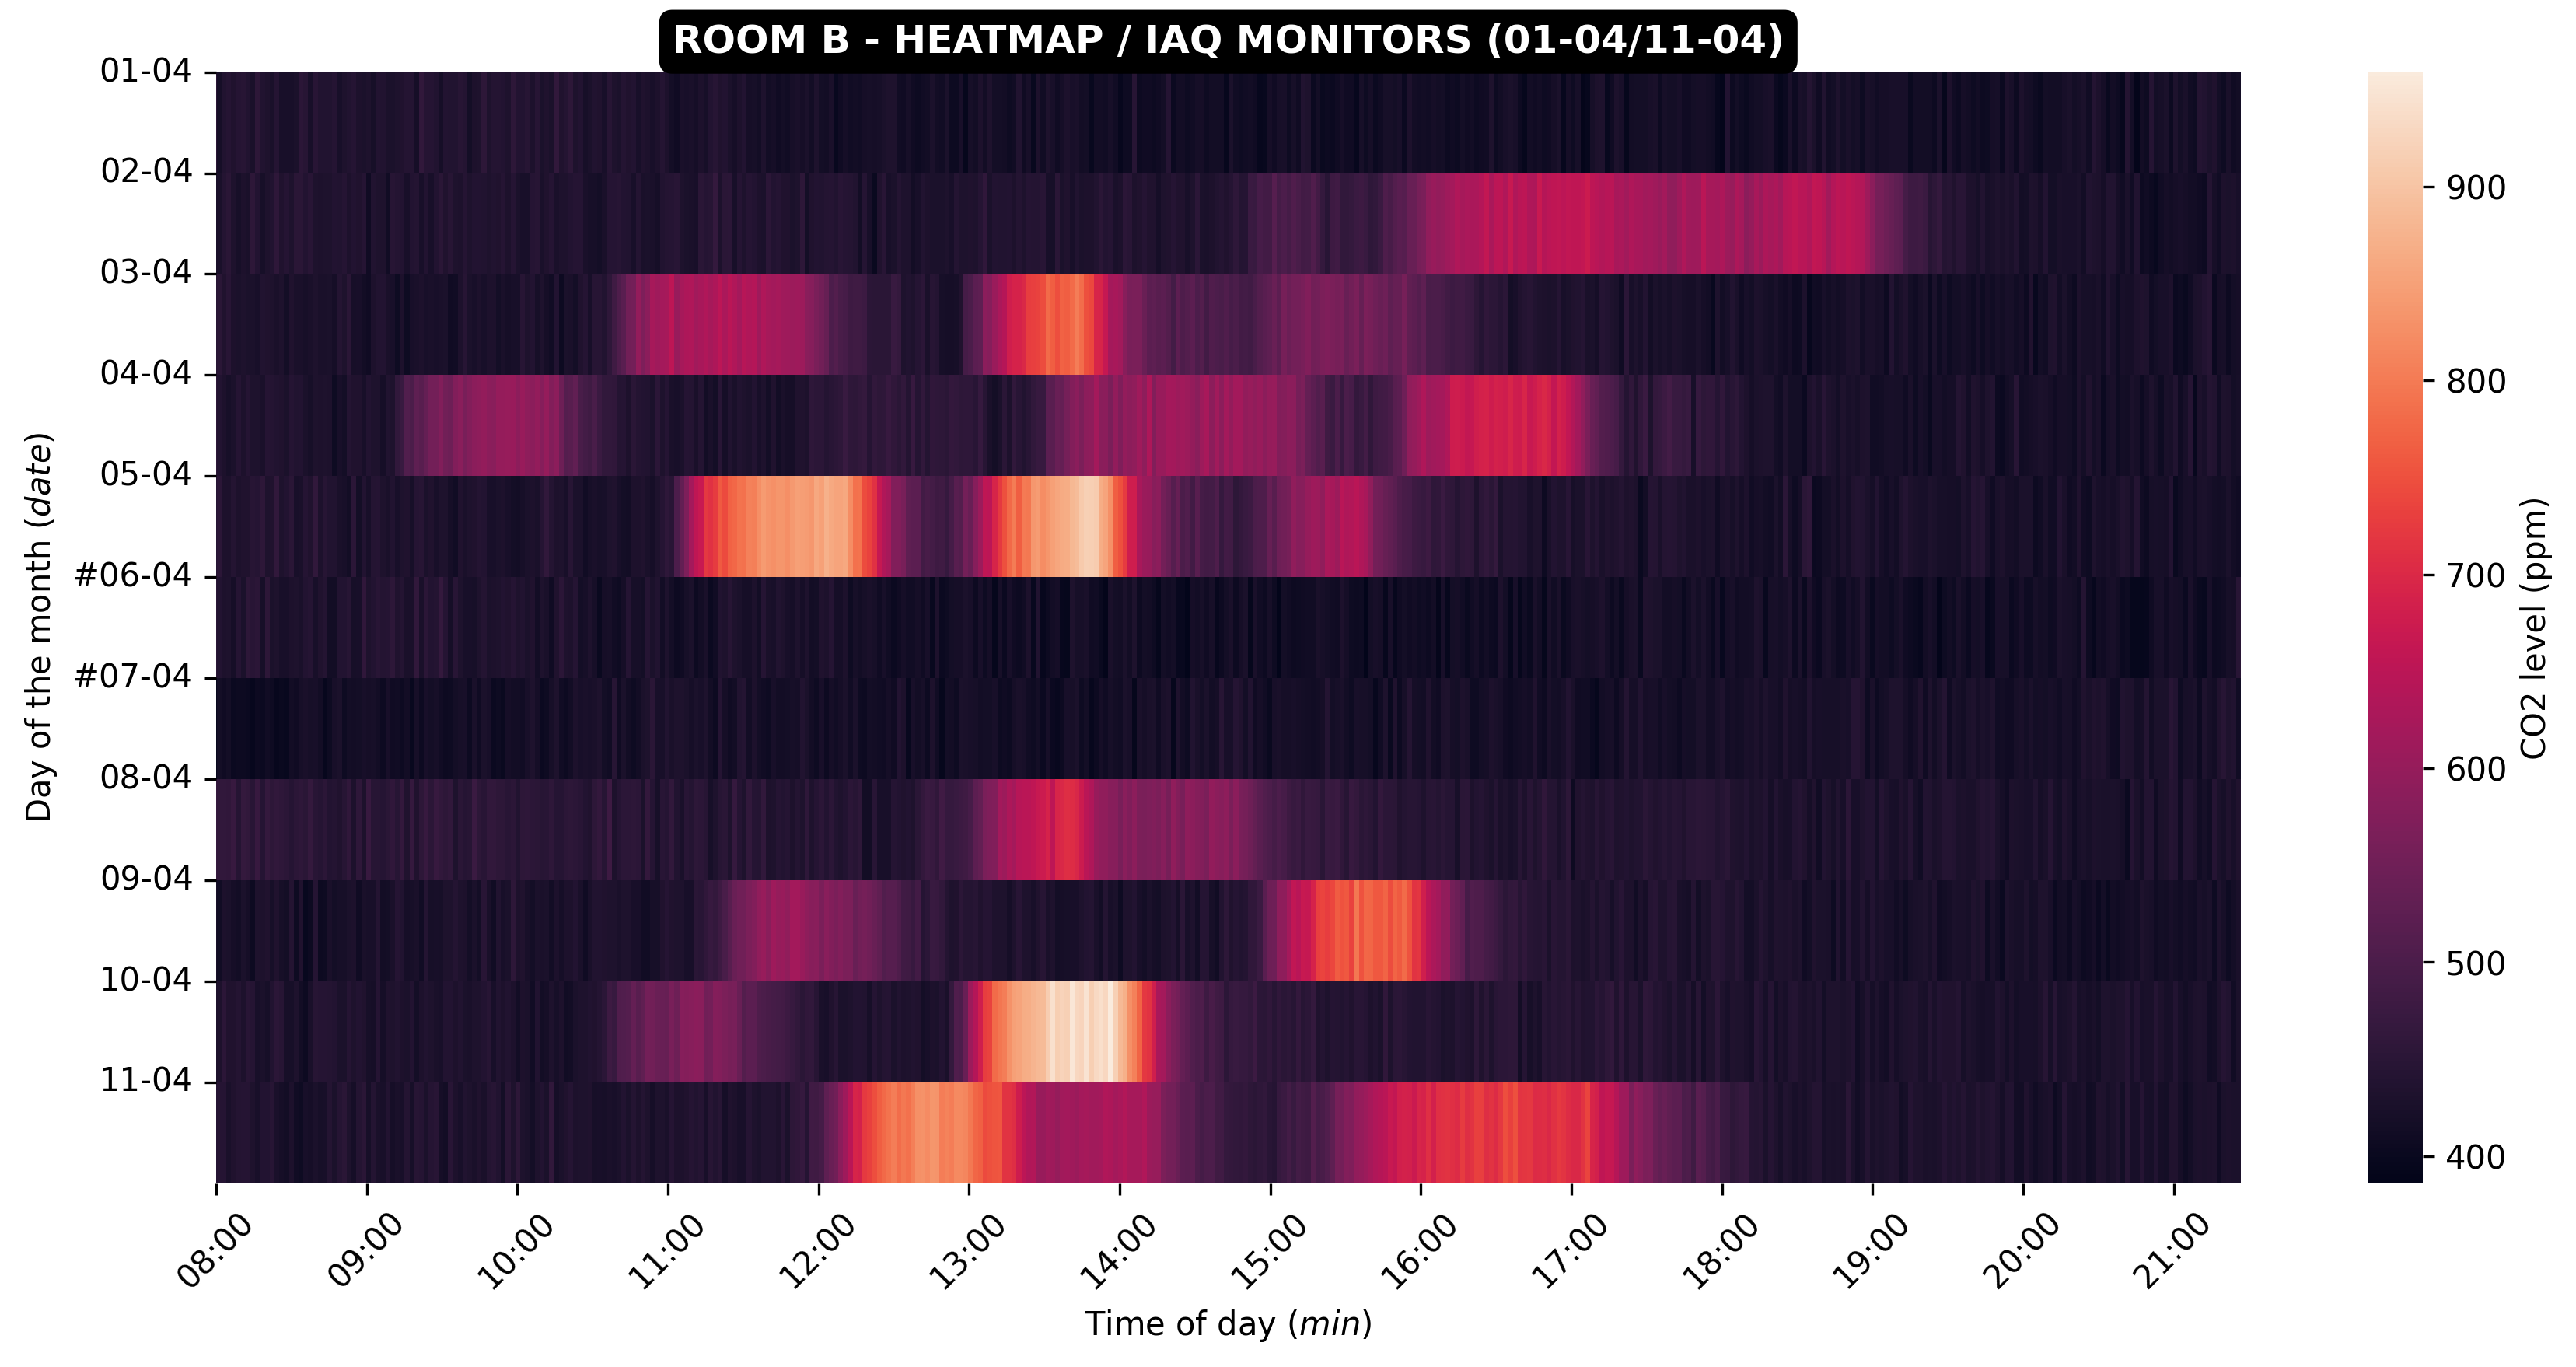
\includegraphics[width=\textwidth]{room-b-monitor-heatmap.png}
        \caption{Heatmap of ten days of monitoring in Room B}
        \label{fig:monitor-heatmap-b}
    \end{subfigure}
    \caption{IAQ monitoring heatmap CO2 concentrations of the sample ten days based on the opening hours of the building}
    \label{fig:monitoring-heatmap}
\end{figure}

\newpage

\section{Evaluation Interviews}
\label{appendix:evaluation}

Semi-structured interview outline for the evaluation sessions conducted in English where the prototype is installed in situ within a meeting room on the sixth floor of the Lab42 building. The questions and structure below served as a guideline for the interviews and follow-up questions were asked based on the responses of the participants.

\vspace{5pt}

\textit{\textbf{Introduction:}}

First of all, thank you for participating in this evaluation study researching indoor air quality and testing the proof-of-concept prototype Bluebird. This evaluation study consists of three parts, 1) a semi-structured interview with questions about your activity within this building and notion of IAQ 2) a usability test of the functioning and perception of the prototype and 3) a score questionnaire rating the prototype on several properties. As a participant you cannot do anything wrong, this is a prototype so only it can malfunction. During the testing I will ask you to think out loud and will ocassionaly ask follow-up questions. Pilot tests of this evaluation session indicated that it will take \~50 minutes. \\

\textit{\textbf{Informed Consent:}}

Your participation will be fully anonymized. If you agree, I will record this meeting for archival purposes and transcription. If you feel uncomfortable at any point during this evaluation session, please feel free to stop it at any point. If you don't want to answer any specific questions feel free to state that you would like to skip and I will move on to the next question.

\begin{table}[htbp]
    \captionsetup{justification=raggedright,singlelinecheck=false}
    \raggedright \textbf{Question-set 1:} \textit{Demographics and roles} \\
    \label{tab:column_widths}
    \raggedright \textbf{Introduction:} First I'm going to ask some questions about your demographics and use of this building.
    \begin{tabularx}{\textwidth}{|p{0.25\textwidth}|X|}
        \hline
        \textbf{Description} & \textbf{Questions (open-ended)} \\
        \hline
        Demographics for sample size & \textbf{Q1:} What is your age? \\
        & \textbf{Q2:} What gender do you identify with? \\
        & \textbf{Q3:} What is your nationality? \\
        & \textbf{Q4:} What is your level of education? \\
        \hline
        Role of the occupant & 
        \textbf{Q5:} What do you do in daily life for work? \\
        & \textbf{Q6:} How would you describe your role within this building? \\
        & \textbf{Q7:} Where are you usually stationary located in the building? \\
        \hline
    \end{tabularx}
\end{table}

\vspace{-10pt}

\begin{table}[htbp]
    \captionsetup{justification=raggedright,singlelinecheck=false}
    \raggedright \textbf{Question-set 2:} \textit{Activity and frequency} \\
    \label{tab:column_widths}
    \raggedright \textbf{Introduction:} Now on to some questions about your activity within this building and how you use the meeting rooms.
    \begin{tabularx}{\textwidth}{|p{0.25\textwidth}|X|}
        \hline
        \textbf{Description} & \textbf{Questions (open-ended)} \\
        \hline
        Frequency of activity & \textbf{Q8:} How often do you use this building for various activities? \\
        & \textbf{Q9:} For what types of activities do you usually use the building for? \\
        \hline
        Frequency of meetings & \textbf{Q10:} On average how many meetings do you have per week? \\
        & \textbf{Q11:} On average how long is a typical meeting you attend? \\
        & \textbf{Q12:} What locations do you typically use for your meetings? \\
        \hline
    \end{tabularx}
\end{table}

\vspace{-10pt}

\begin{table}[htbp]
    \captionsetup{justification=raggedright,singlelinecheck=false}
    \raggedright \textbf{Question-set 3:} \textit{Notion of Indoor Air Quality (IAQ)} \\
    \label{tab:column_widths}
    \raggedright \textbf{Introduction:} Lastly some questions about your notion of indoor air quality as a baseline.
    \begin{tabularx}{\textwidth}{|p{0.25\textwidth}|X|}
        \hline
        \textbf{Description} & \textbf{Questions (open-ended)} \\
        \hline
        IAQ awareness & \textbf{Q11:} How aware are you of the current IAQ in this space? 
        \newline
        \textbf{Q12:} How do you perceive the IAQ in this space? \\
        \hline
        Cognitive and health & \textbf{Q13:} Have you ever experienced cognitive symptoms related to IAQ in a meeting room? 
        \newline
        \textbf{Q14:} Have you ever experienced health symptoms related to IAQ in a meeting room?  \\
        \hline
    \end{tabularx}
\end{table}

\newpage

\section{Usability tests}
\label{appendix:usability}

For the usability tests, we shifted attention towards the prototype that was installed in the meeting room. In all sessions, the researcher and occupants stood up and walked towards the prototype. The occupants were allowed to touch the prototype and observe its movements.
\vspace{5pt}

\textit{\textbf{Introduction:}}

We will move on to testing the prototype. Please imagine you are an occupant having a meeting in the space (meeting room) we are currently in. As you might have noticed on the wall hanging from the ceiling, a prototype of a physical artifact is hung up.\\

\begin{table}[htbp]
    \captionsetup{justification=raggedright,singlelinecheck=false}
    \raggedright \textbf{Question-set 1:} \textit{Understanding of the prototype (learnability)} \\
    \raggedright \textbf{Introduction:} To gather some first impressions I would like to get some description of the prototype based on your view of it.
    \label{tab:column_widths}
    \begin{tabularx}{\textwidth}{|p{0.25\textwidth}|X|}
        \hline
        \textbf{Description} & \textbf{Questions (open-ended)} \\
        \hline
        Description of prototype & \textbf{Q1:} Could you describe in your own words what the physical artifact is? \\
        \hline
        Look and feel & 
        \textbf{Q2:} What do you think of the overall design of the physical artifact? \\
        \hline
        Use of materials & 
        \textbf{Q3:} What do you think of the materials the physical artifact is made of? \\
        \hline
        Communicative properties & 
        \textbf{Q4:} What properties do you think the data physicalization communicates?\\
        \hline        
    \end{tabularx}
\end{table}

\vspace{-10pt}

\begin{table}[htbp]
    \captionsetup{justification=raggedright,singlelinecheck=false}
    \raggedright \textbf{Question-set 2:} \textit{Self-reflection of data insight (memorability)} \\
    \raggedright \textbf{Introduction:} I want to gain insight into how likely you are to take preventative action based on data insights.
    \label{tab:column_widths}
    \begin{tabularx}{\textwidth}{|p{0.25\textwidth}|X|}
        \hline
        \textbf{Description} & \textbf{Questions (open-ended)} \\
        \hline
        Behavourial change & 
        \textbf{Q5:} How and to what extent do you think your awareness of IAQ changes? \\
        & \textbf{Q6:} How willingly are you to take preventative action based on the data insights the artifact provides? \\
        \hline
    \end{tabularx}
\end{table}

\vspace{-10pt}


\begin{table}[htbp]
    \captionsetup{justification=raggedright,singlelinecheck=false}
    \raggedright \textbf{Question-set 3:} \textit{Design improvements and further development} \\
    \raggedright \textbf{Introduction:} After interacting with the prototype for a bit. This usability test concludes with suggestions for design improvements.
    \label{tab:column_widths}
    \begin{tabularx}{\textwidth}{|p{0.25\textwidth}|X|}
        \hline
        \textbf{Description} & \textbf{Questions (open-ended)} \\
        \hline
        Good characteristics & \textbf{Q7:} What do you think is the best aspect of this data physicalization, and why? \\
        \hline
        Design improvements & \textbf{Q8:} What do you think needs most improvement of the design, and why? \\
        \hline
        Further development & \textbf{Q9:} Is there anything that you would wish to be considered further development of the prototype? \\
        \hline
    \end{tabularx}
\end{table}

\section{Effectiveness scores}
\label{appendix:effectiveness}

The occupant and researcher sit down on the table again and the occupant is handed the computer or phone of the researcher to fill in an online statement questionnaire on Qualtrics with Likert scales. \\

\raggedright \textit{\textbf{Introduction:}} \\ The last part is an online score rating statement and hypothesis about the prototype. 

\vspace{5pt}

\begin{table}[htbp]
    \captionsetup{justification=raggedright,singlelinecheck=false}
    \raggedright \textbf{Effectiveness scores} \textit{Rating statements and hypothesis} \\
    \label{tab:column_widths}
    \raggedright \textbf{Introduction:} Please rate the following statements based on the five-point scale (likert)
    \begin{tabularx}{\textwidth}{|p{0.25\textwidth}|X|}
        \hline
        \textbf{Description} & \textbf{Statements (Likert-scale 5 points 1: Strongly disagree 5: Strongly agree)} \\
        \hline        
        \hline
        Attitute towards using & \textbf{S1:} I enjoyed viewing the data physicalization and interacting with the prototype \\
        \hline
        Perceived Ease of use & \textbf{S2:} I thought the data physicalization was easy to use and interpret \\
        \hline
        Learnability of data & \textbf{S3:} I would imagine that most people would learn to use the data physicalization very quickly \\
        \hline
        Perceived Usefulness & \textbf{S4:} I derived insights into state of the indoor air quality based on the data physicalization \\
        \hline
        Behavioural Intention & \textbf{S5:} I likely will change my behaviour and take preventive measures based on the data insights \\        
        \hline
    \end{tabularx}
\end{table}

\textit{\textbf{Final remarks:}}

Do you have any other final remarks you want to share about the prototype?  If not, this marks the end of this evaluation session. Thank you so much for your valuable time, insights and feedback. If you want any more information or the published results of this research please contact me.\\

\newpage

\section{Evaluation participant sample}
\label{appendix:participants}

Sample size and demographics (see \hyperref[table:design_improvements]{Table \ref{table:design_improvements}}) of the participants who participated with their expertise and building activity.

\begin{table}[h!]
\centering
\begin{tabular}{| p{2cm} | p{1.5cm} | p{1cm} | p{3cm} | p{2cm} | p{3cm} | p{3cm} |}
\hline
\textbf{Participant} & \textbf{Gender} & \textbf{Age} & \textbf{Expertise} & \textbf{Education} & \textbf{Days in building} & \textbf{Working Space} \\ 
\hline
P1 & Male & 35 & HCI/Researcher & PhD & 3 days a week & Lab Office Space \\ 
\hline
P2 & Male & 28 & Software Engineer & Master & 5 days a week & Shared Office \\ 
\hline
P3 & Female & 30 & UX Designer & Bachelor & 4 days a week & Open Workspace \\ 
\hline
P4 & Male & 32 & Data Scientist & Master & 2 days a week & Private Office \\ 
\hline
P5 & Female & 25 & Research Assistant & Bachelor & 1 day a week & Lab Office Space \\ 
\hline
\end{tabular}
\caption{Participants sample of the Evaluation Sessions demographics}
\label{table:participants}
\end{table}


\section{Design improvements and recommendations}
\label{appendix:improvements}

Coding of main design improvements and recommendations (see \hyperref[table:participants]{Table \ref{table:participants}}) based on the feedback during the usability testing.


\begin{table}[h!]
\centering
\begin{tabular}{| p{1.5cm} | p{4cm} | p{8cm} | p{3cm} |}
\hline
\textbf{Coding} & \textbf{Design Improvements (DI)} & \textbf{Design Recommendations (DR)} & \textbf{Category} \\ 
\hline
DI-1 & Light as material and circular data & An instruction board is recommended to help people understand the visualization & Material type \\ 
\hline
DI-2 & Improved color contrast for better readability & Use high-contrast colors for text and background to enhance readability & Visual design \\ 
\hline
DI-3 & Interactive elements for user engagement & Implement interactive features such as clickable icons to engage users & User Interaction \\ 
\hline
DI-4 & Simplified navigation menu & Provide a simplified and intuitive navigation menu for ease of use & Navigation \\ 
\hline
\end{tabular}
\caption{Design Improvements and Recommendations}
\label{table:design_improvements}
\end{table}

\section{Statement likert scores}
\label{appendix:implications}

Individual results of the statement scores in a table (see \hyperref[table:participant_scores]{Table \ref{table:participant_scores}}) and bar chart plot (see \hyperref[fig:survey-statement-scores]{Figure \ref{fig:survey-statement-scores}}).

\begin{table}[h!]
\centering
\begin{tabular}{| p{2cm} | >{\centering\arraybackslash}p{2cm} | >{\centering\arraybackslash}p{2cm} | >{\centering\arraybackslash}p{2cm} | >{\centering\arraybackslash}p{2cm} | >{\centering\arraybackslash}p{2cm} | >{\centering\arraybackslash}p{3cm} |}
\hline
\textbf{Participant} & \textbf{S1} & \textbf{S2} & \textbf{S3} & \textbf{S4} & \textbf{S5} & \textbf{Average Score} \\ 
\hline
P1 & 3 & 5 & 2 & 4 & 1 & 3.00 \\ 
\hline
P2 & 4 & 3 & 4 & 2 & 5 & 3.60 \\ 
\hline
P3 & 5 & 2 & 3 & 5 & 4 & 3.80 \\ 
\hline
P4 & 2 & 4 & 1 & 3 & 2 & 2.40 \\ 
\hline
P5 & 1 & 3 & 5 & 4 & 3 & 3.20 \\ 
\hline
\textbf{Average} & \textbf{3.00} & \textbf{3.40} & \textbf{3.00} & \textbf{3.60} & \textbf{3.00} & \textbf{3.20} \\ 
\hline
\textbf{Variance} & \textbf{2.50} & \textbf{1.70} & \textbf{2.50} & \textbf{1.70} & \textbf{2.00} & \textbf{0.19} \\ 
\hline
\end{tabular}
\caption{Participant Scores, Averages, and Variance}
\label{table:participant_scores}
\end{table}

\begin{figure}[H]
    \centering
    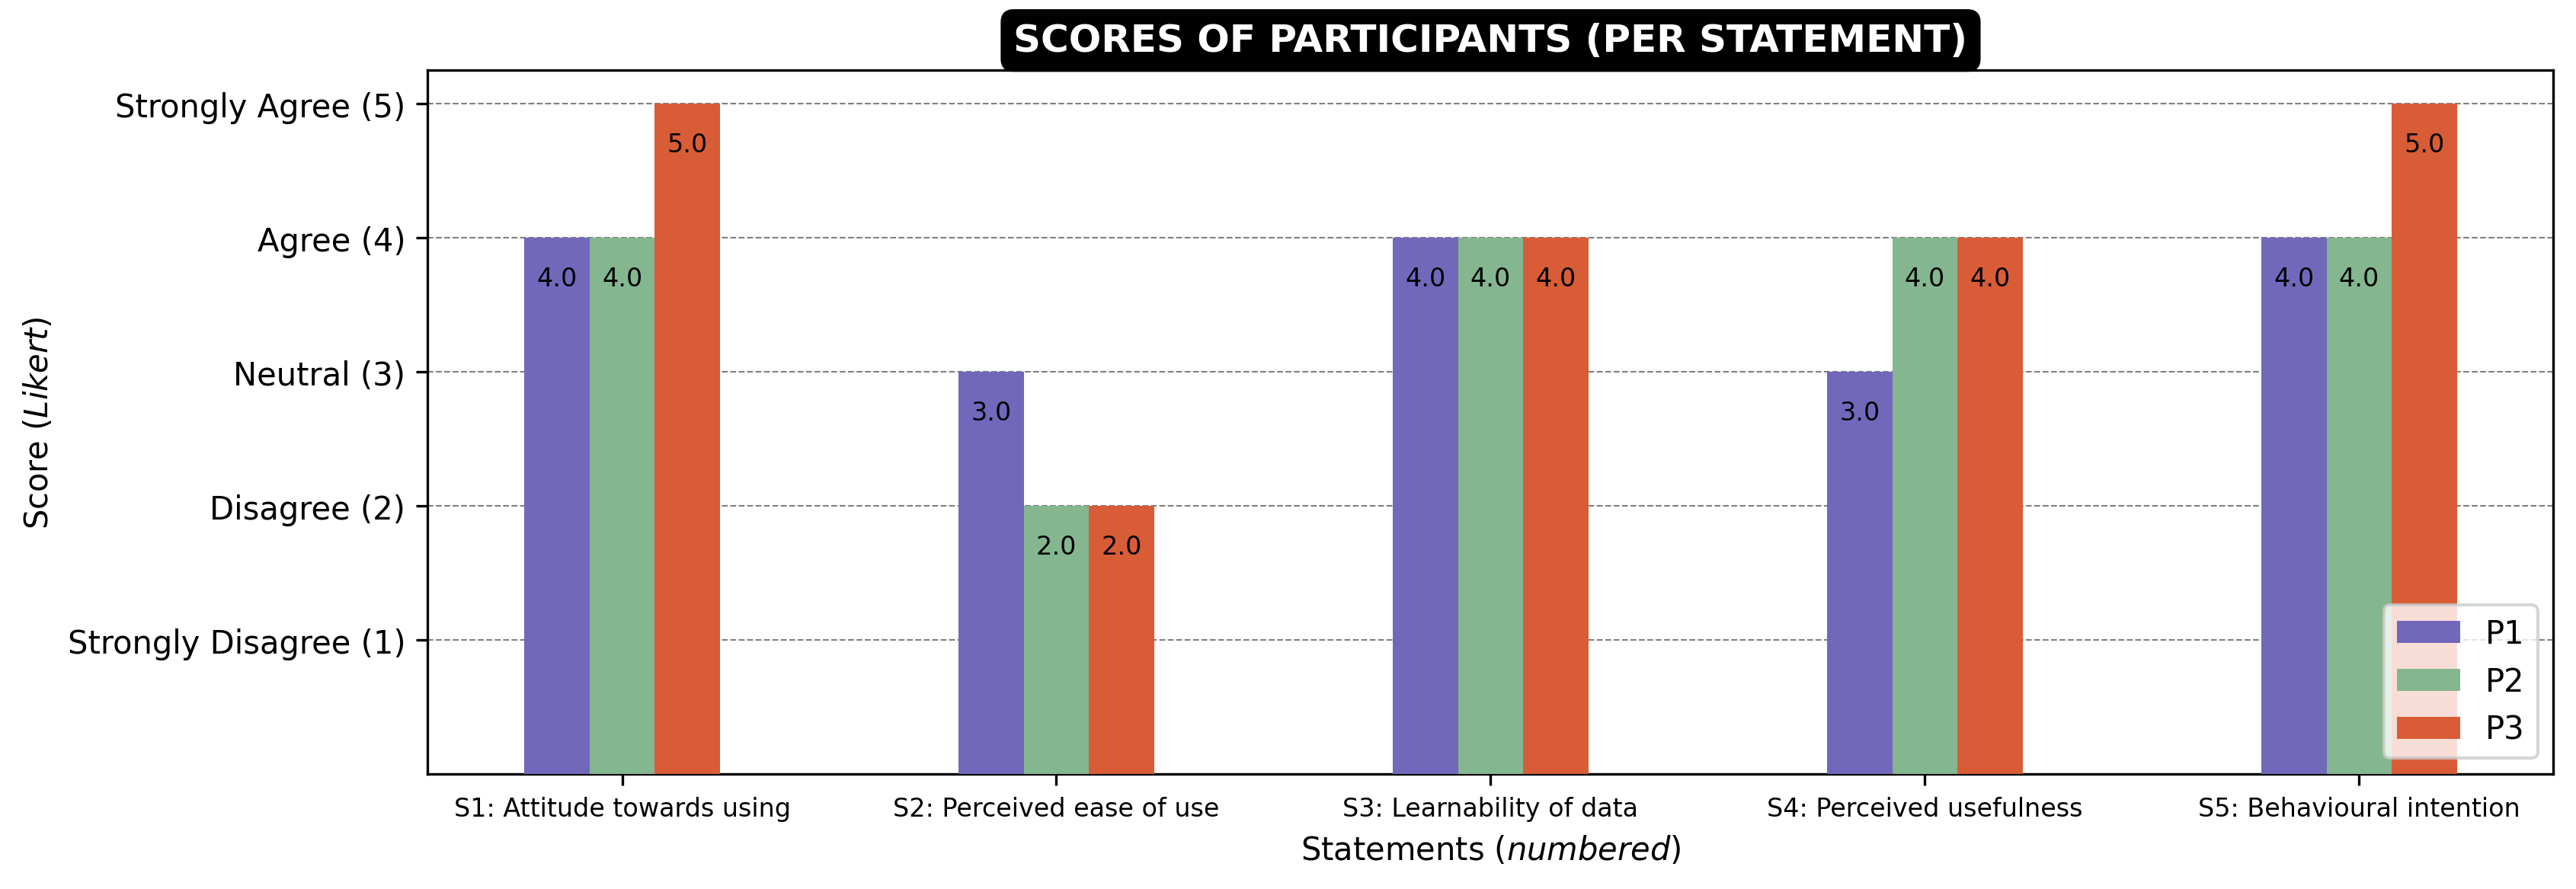
\includegraphics[width=0.55\paperwidth]{statement-scores-per-statement.png}
    \caption{5-point likert-scales of participants per statement}
    \label{fig:survey-statement-scores}
\end{figure}

\newpage

\section{Concept diagrams}
\label{appendix:conceptdiagrams}

Design diagrams (see \hyperref[fig:concept-one]{Figure \ref{fig:concept-one}}, \hyperref[fig:concept-two]{Figure \ref{fig:concept-two}}, \hyperref[fig:concept-three]{Figure \ref{fig:concept-three}}) of the brainstormed concepts in medium-fi sketches that show the component breakdown and interaction states.\\

\vspace{1em}

\textbf{Concept-1: Desk Planter (Aspen)}\\
A desk planter or tree in the corner of the room with soil in it.Follows the organic growth of a 'seed' of a flower or tree from seed to sprouts to full flower. The better the air quality the more or faster the plant grows. The movement of the leaves can indicate the wind.


\begin{figure}[H]
    \centering
    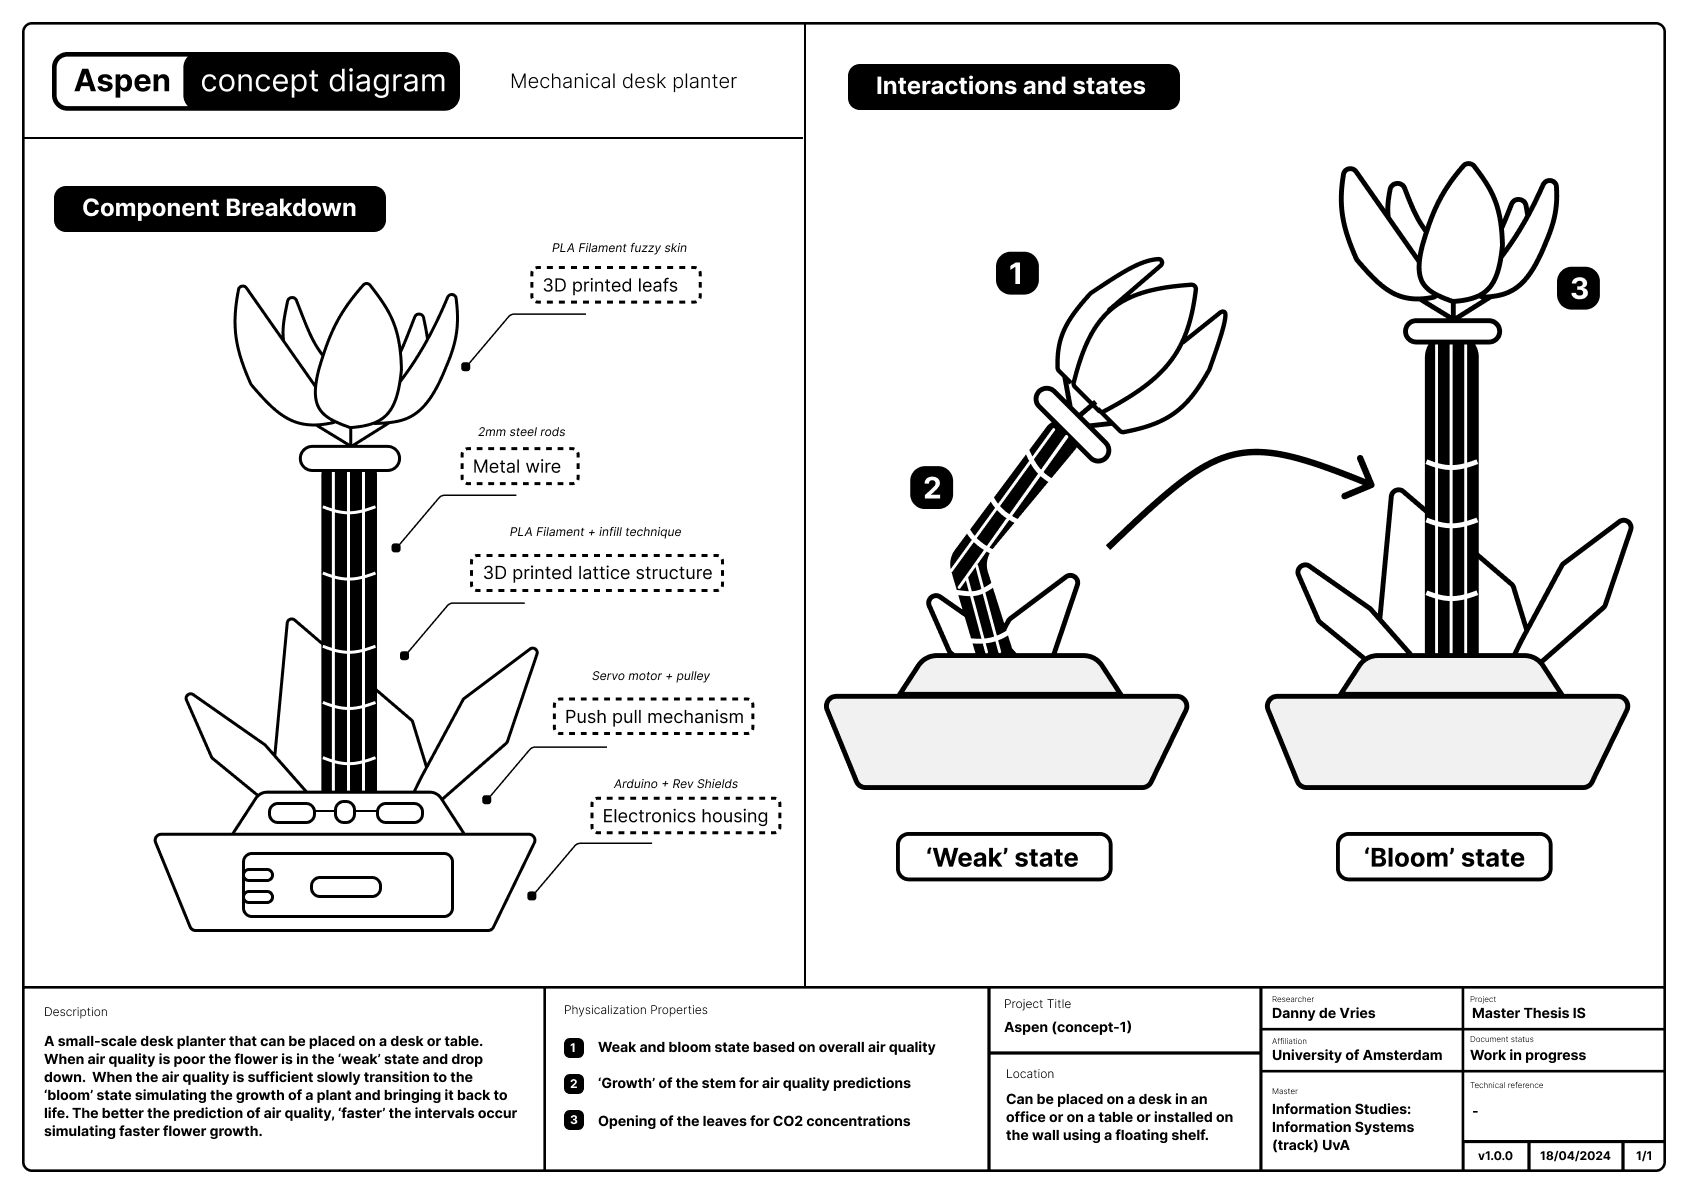
\includegraphics[width=0.5\paperwidth]{Concept-1_Aspen_Design_Diagram.jpg}
    \caption{Design diagram of concept one (Aspen)}
    \label{fig:concept-one}
\end{figure}

\textbf{Concept-2: Hanging Sculpture (Bluebird)}\\
A hanging planter-type set-up with strings that 'grow' from the ceiling. Fresh air moves the strings. People can walk by, and feel the material (e.g. humidity). Allows most interactivity. Taking inspiration from kinetic sculptures and hanging/floating sculptures.

\begin{figure}[H]
    \centering
    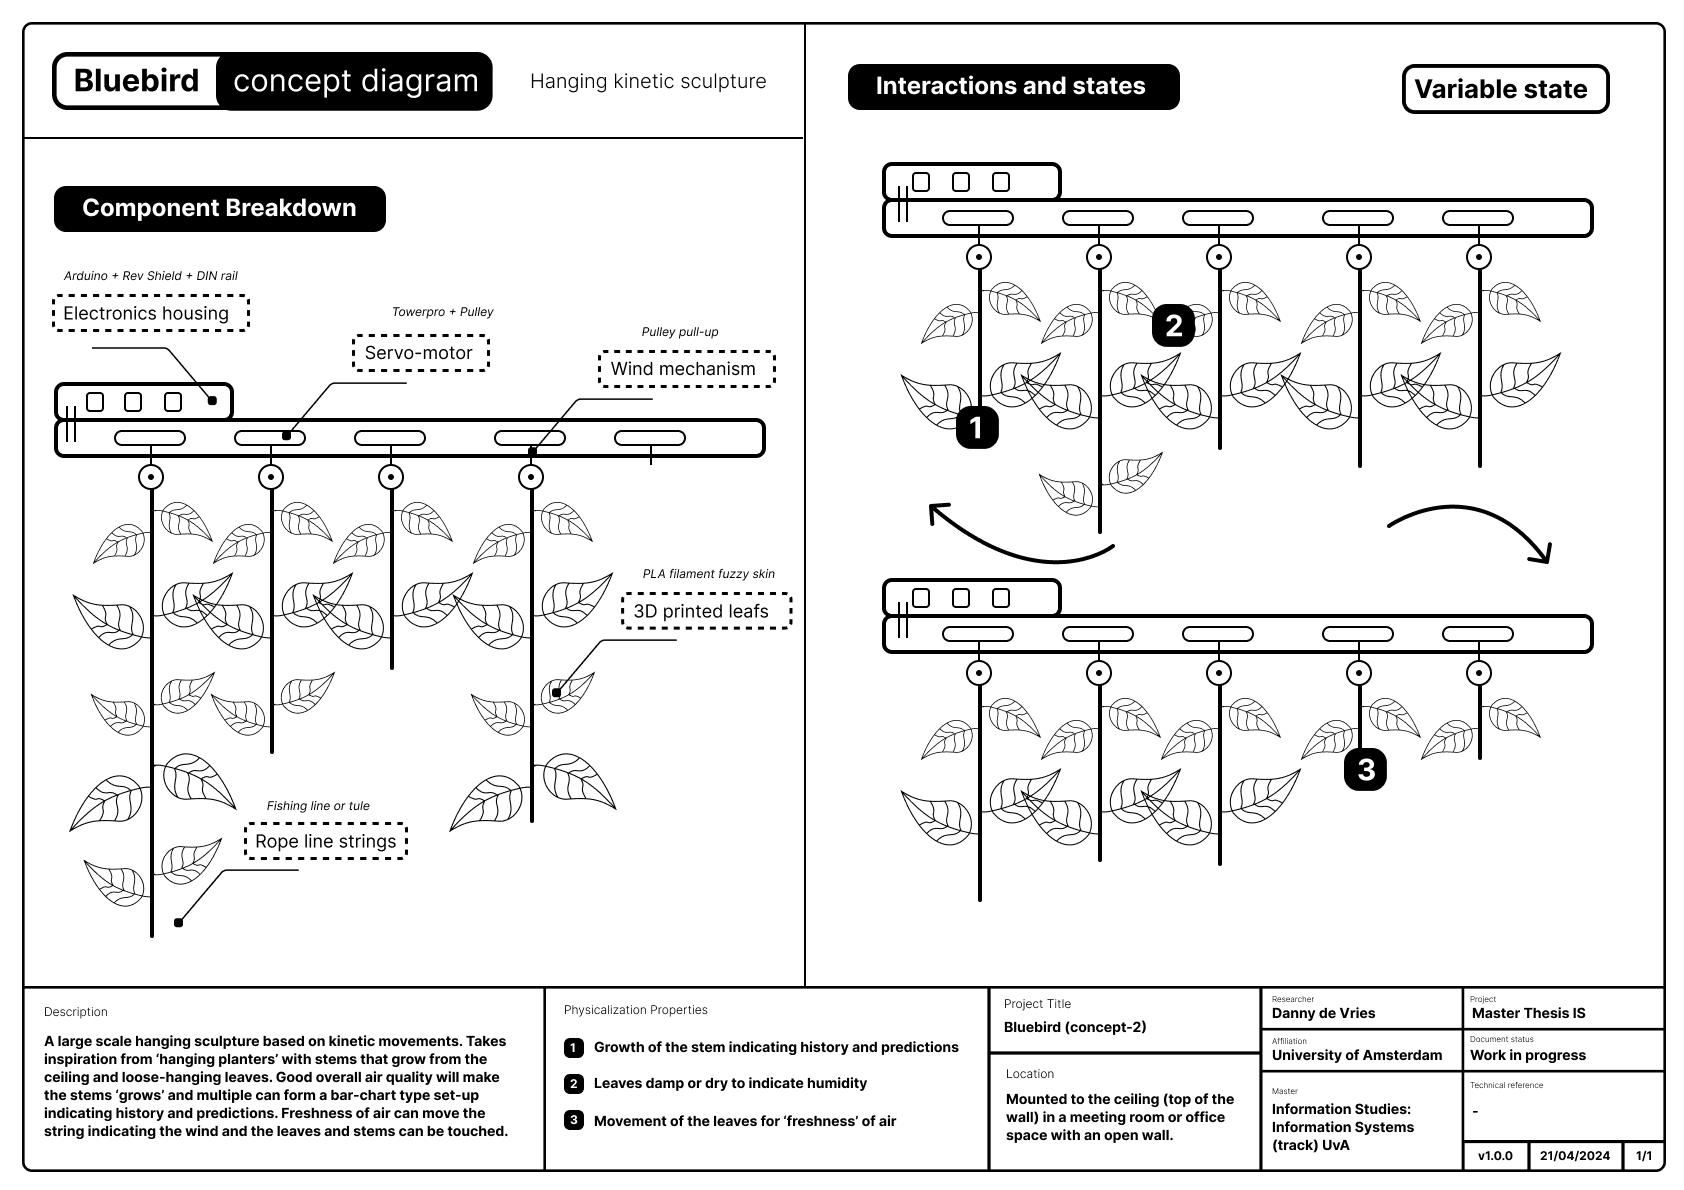
\includegraphics[width=0.5\paperwidth]{Concept-2_Bluebird_Design_Diagram.jpg}
    \caption{Design diagram of concept two (Bluebird)}
    \label{fig:concept-two}
\end{figure}

\newpage

\textbf{Concept-3: Wall Kinetic (Crocus)} \\
A moss-like structure on the wall with flower bulbs embedded. The flowers 'open up' based on better fresh air. Taking inspiration from kinetic sculptures.

\begin{figure}[H]
    \centering
    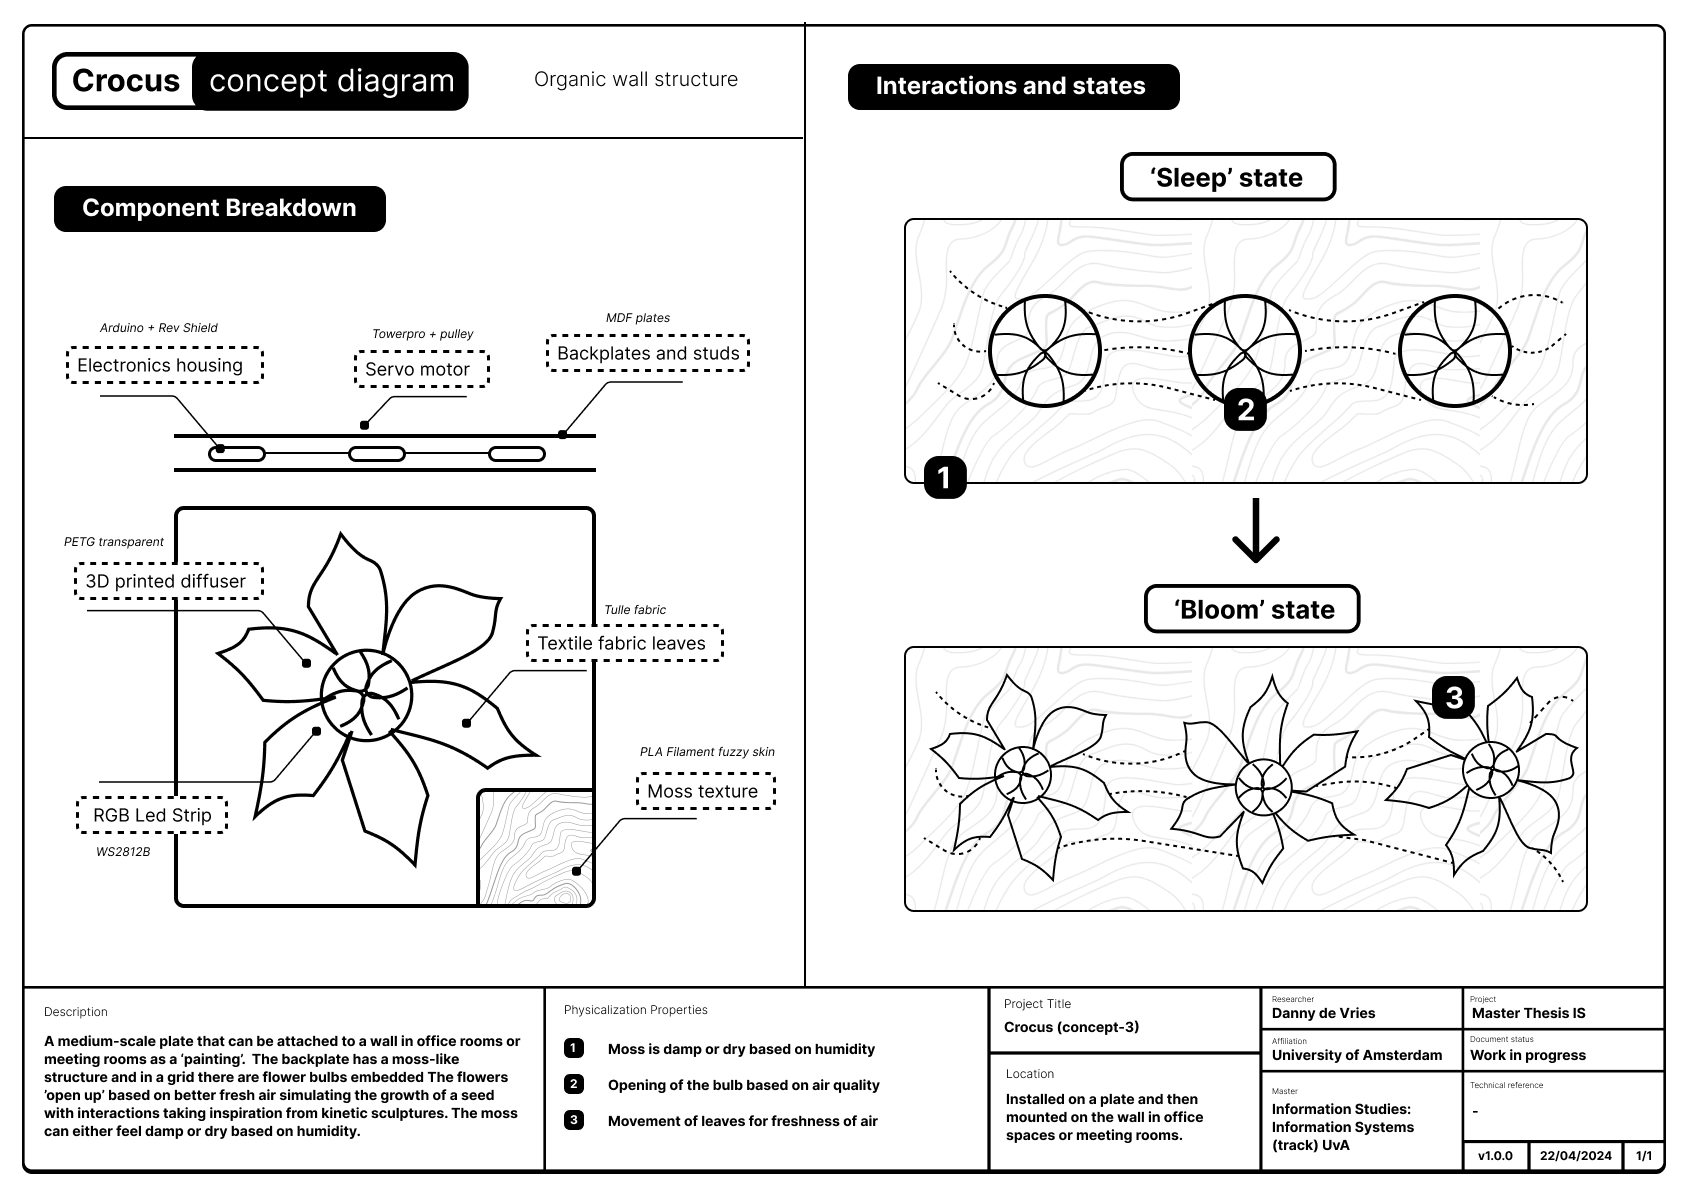
\includegraphics[width=0.5\paperwidth]{Concept-3_Crocus_Design_Diagram.jpg}
    \caption{Design diagram of concept three (Crocus)}
    \label{fig:concept-three}
\end{figure}

\section{Academic Sample Case Studies}
\label{appendix:academic}

In the ideation phase and development of the concept models, an exploration of 10 academic case studies were instrumental in informing the design of the prototype. \hyperref[table:academic-cases]{Table \ref{table:academic-cases}} provides an overview of all these case studies.

\begin{table}[htbp]
\centering
\begin{tabularx}{\textwidth}{|>{\raggedright\arraybackslash}m{1cm}|X|X|>{\raggedright\arraybackslash}m{1cm}|X|X|}
\hline
\textbf{Nr.} & \textbf{Sample} & \textbf{Author(s)} & \textbf{Year} & \textbf{Venue} & \textbf{Reference} \\ \hline
1 & Econundrum & Kim Sauvé et al. & 2020 & ACM & \href{https://dl.acm.org/doi/10.1145/3357236.3395509}{Econundrum} \\ \hline
2 & Caimform & Maxime Daniel et al. & 2019 & HAL & \href{https://hal.science/hal-01976793/document/}{Caimform} \\ \hline
3 & Dataponics & Robert Cercós et al. & 2016 & DEG & \href{http://dataphys.org/list/dataponics-human-vegetal-play/}{Dataponics} \\ \hline
4 & Garden of Eden & Thorsten Kiesl et al. & 2007 & UFG & \href{http://dataphys.org/list/garden-of-eden/}{Garden of Eden} \\ \hline
5 & Pudica & Olivia Seow et al. & 2022 & MIT & \href{https://trackr-media.tangiblemedia.org/publishedmedia/Papers/715-MTA0N/Published/PDF}{Pudica} \\ \hline
6 & ComfortBox & Hamed S. Alavi et al. & 2017 & IFIP & \href{https://doi.org/10.1007/978-3-319-67687-6_16}{ComfortBox} \\ \hline
7 & ComFeel & Ugo Sassi et al. & 2020 & ACM & \href{https://dl.acm.org/doi/10.1145/3432234}{ComFeel} \\ \hline
8 & WindowWall & Patrick Bader et al. & 2020 & ACM & \href{https://doi.org/10.1145/3310275}{WindowWall} \\ \hline
9 & Ambient Influence & Yvonne Rogers et al. & 2010 & ACM & \href{https://dl.acm.org/doi/10.1145/1864349.1864372}{Ambient Influence} \\ \hline
10 & Hilo-wear & Shailin Zong et al. & 2020 & CHI & \href{https://dl.acm.org/doi/10.1145/3334480.3382813}{Hilo-wear} \\ \hline
\end{tabularx}
\caption{Overview of the 10 academic case studies used for the ideation phase and concept models.}
\label{table:academic-cases}
\end{table}

\newpage

\section{Non-academic Sample Case Studies}
\label{appendix:nonacademic}

In the ideation phase and development of the concept models, an exploration of 24 non-academic case studies were instrumental in informing the design of the prototype. \hyperref[tab:non-academic-cases]{Table \ref{tab:non-academic-cases}} provides an overview of all these case studies.

\begin{table}[htbp]
\centering
\begin{tabularx}{\textwidth}{|>{\raggedright\arraybackslash}m{1cm}|X|X|>{\raggedright\arraybackslash}m{1cm}|X|X|}
\hline
\textbf{Nr.} & \textbf{Sample} & \textbf{Creator(s)} & \textbf{Year} & \textbf{Venue} & \textbf{Reference} \\ \hline
1 & Birdie Design & Birdie Design & 2024 & non-academic & \href{https://www.birdie.design/}{Birdie Design} \\ \hline
2 & Tree of Ténéré & Studio Drift & 2017 & non-academic & \href{https://studiodrift.com/work/tree-of-tenere/}{Studio Drift} \\ \hline
3 & Petal Clouds & ART+COM & 2018 & non-academic & \href{https://artcom.de/en/?project=petalclouds}{ART+COM} \\ \hline
4 & Electro Magnetic Field & Jennifer Allora & 2022 & non-academic & \href{https://arkive.net/gallery/electromagnetic-field}{Arkive} \\ \hline
5 & Wind 3.0 & Studio Roosegaarde & 2011 & non-academic & \href{https://www.studioroosegaarde.net/project/wind-3-0}{Studio Roosegaarde} \\ \hline
6 & Floralis Generica & Eduardo Catalano & 2002 & non-academic & \href{https://en.wikipedia.org/wiki/Floralis_Generica}{Plaza Unidas} \\ \hline
7 & Flylight & Studio Drift & 2013 & non-academic & \href{https://studiodrift.com/work/flylight/}{Studio Drift} \\ \hline
8 & Spectra-2 & FIELD.IO & 2015 & non-academic & \href{https://field.io/explorations/spectra-2}{FIELD.IO} \\ \hline
9 & Meadow & Studio Drift & 2023 & non-academic & \href{https://studiodrift.com/work/meadow/}{Studio Drift}  \\ \hline
10 & Pet Lamp & Álvaro Catalán & 2024 & non-academic & \href{https://www.petlamp.org/}{Pet Lamp} \\ \hline
11 & Living map & Sigitas Guzauskas & 2018 & non-academic & \href{https://www.behance.net/gallery/68572509/LIVING-MAP}{Living map} \\ \hline
12 & Harassment plants & Nazareno Andrade & 2022 & non-academic & \href{https://luizaugustomm.github.io/pages/harassment-plants.html}{Harassment plants} \\ \hline
13 & Popsicles of Pollution & Hung Yi-Chen, & 2017 & non-academic & \href{https://www.theguardian.com/cities/gallery/2017/sep/01/popsicles-pollution-ice-lollies-taiwan-taipei-contaminated-waterways}{Popsicles of Pollution} \\ \hline
14 & Yellow Dust & C+arquitectos & 2017 & non-academic & \href{http://yellowdust.intheair.es/}{Yellow Dust} \\ \hline
15 & Touching air & Miriam Quick & 2015 & non-academic & \href{https://www.stefanieposavec.com/airtransformed}{Touching air} \\ \hline
16 & Physical Weather Display & Ken Kawamoto & 2015 & non-academic & \href{https://www.boredpanda.com/weather-forecast-box-tempescope-ken-kawamoto/}{Physical Weather Display} \\ \hline
17 & Inequalities Quipu & Ewa Tuteja & 2021 & non-academic & \href{https://tuteja.info/inequalities-quipu/}{Inequalities Quipu} \\ \hline
18 & Summer in the city & Carola Bartsch & 2015 & non-academic & \href{https://www.carolabartsch.ch/en/projects/dataviz}{Summer in the city} \\ \hline
19 & WeatherWindow & Tim Dye & 2014 & non-academic & \href{http://dataphys.org/list/weatherwindow/}{WeatherWindow} \\ \hline
20 & Point cloud & James Leng & 2012 & non-academic & \href{https://www.jamesleng.net/pointcloud/}{Point cloud} \\ \hline
21 & Tele-present water & David Bowen & 2011 & non-academic & \href{https://www.dwbowen.com/telepresentwater/}{Tele-present water} \\ \hline
22 & Real-time Warning & Rodrigo Medeiros & 2012 & non-academic & \href{https://vimeo.com/35520114}{Real-time Warning} \\ \hline
23 & airFIELD & Dan Goods & 2012 & non-academic & \href{http://dataphys.org/list/ecloud-airfield-ambient-airport-visualizations/}{airFIELD} \\ \hline
24 & Shanghai Spheres & Michael Tait & 2018 & non-academic & \href{https://www.taittowers.com/work?sort=newest}{Shanghai Spheres} \\ \hline
\end{tabularx}
\caption{Overview of the 24 non-academic case studies used for the ideation phase and concept models.}
\label{tab:non-academic-cases}
\end{table}

\section{Fabrication Techniques}
\label{appendix:fabrication}

In the ideation phase and development of the concept models, an exploration of 4 academic and 6 non-academic case studies were instrumental in informing the fabrication of the prototype. \hyperref[tab:fabrication-cases]{Table \ref{tab:fabrication-cases}} provides an overview of all these case studies.

\begin{table}[!htbp]
\centering
\begin{tabularx}{\textwidth}{|>{\raggedright\arraybackslash}m{1cm}|X|X|>{\raggedright\arraybackslash}m{1cm}|X|X|}
\hline
\textbf{Nr.} & \textbf{Sample} & \textbf{Author(s)} & \textbf{Year} & \textbf{Venue} & \textbf{Reference} \\ \hline
1 & FibeRobo & Jack Forman et al. & 2023 & MIT Media Lab (TGM) & \href{https://trackr-media.tangiblemedia.org/publishedmedia/Papers/728-MTA2O/Published/PDF}{TGM} \\ \hline
2 & DefeXtiles & Jack Forman et al. & 2020 & MIT Media Lab (TGM) & \href{https://trackr-media.tangiblemedia.org/publishedmedia/Papers/703-MTAyN/Published/PDF}{TGM} \\ \hline
3 & Cilllia & Jifei Ou et al. & 2016 & MIT Media Lab (TGM) & \href{https://trackr-media.tangiblemedia.org/publishedmedia/Papers/703-MTAyN/Published/PDF}{TGM} \\ \hline
4 & UniMorph & Felix Heiberg et al. & 2015 & MIT Media Lab (TGM) & \href{https://trackr-media.tangiblemedia.org/publishedmedia/Papers/703-MTAyN/Published/PDF}{TGM} \\ \hline
5 & Geometric Floating Fabric & Billie Ruben & 2020 & non-academic & \href{https://www.printables.com/en/model/42342-geometric-floating-fabric-printed-necklace-by-bill}{Printables} \\ \hline
6 & Print On Fabric & Damien Jorrand & 2021 & non-academic & \href{https://than.gs/m/14347}{Thangs} \\ \hline
7 & Nasa Fabric Mk3 & John Bowler & 2018 & non-academic & \href{https://www.thingiverse.com/thing:3095799}{Thingiverse} \\ \hline  
8 & Servo Flower & Job Smolders & 2018 & non-academic & \href{https://pinshape.com/items/41182-3d-printed-servo-flower}{Pinshape} \\ \hline
9 & Multiuse Flexible Fabric & Posix & 2024 & non-academic & \href{https://www.printables.com/model/88579-multiuse-flexible-fabric}{Printables} \\ \hline
10 & Leaf Decorative Holder & Trilobyte3D & 2022 & non-academic & \href{https://www.printables.com/model/230363-leaf-drink-coasters-with-decorative-plant-holder}{Printables} \\ \hline
\end{tabularx}
\caption{Overview of the 4 academic and 6 non-academic sample case studies used as inspiration for fabrication of the prototype.}
\label{tab:fabrication-cases}
\end{table}

\end{appendices}